\documentclass[UTF8,a4paper,11pt]{article}

\usepackage{ctex} 
\usepackage{fancyhdr}
\usepackage{multicol} 
\usepackage{lastpage} 
\usepackage{geometry} 
\usepackage{titlesec} 
\usepackage{mathrsfs}
\usepackage{graphicx}
\usepackage{epstopdf}
\usepackage{ulem}
\usepackage{amsmath}
\usepackage[subfigure,AllowH]{graphfig} 
\usepackage{listings}
\usepackage[usenames,dvipsnames]{xcolor}

\geometry{left=3cm,right=3cm,top=2.5cm,bottom=2.5cm}
\renewcommand{\baselinestretch}{1.5}
\pagestyle{fancy}
\fancyhf{}
\fancyhead[C]{武汉理工大学《单片机应用设计》报告}   %页眉居中,显示节标题名
\fancyfoot[C]{\thepage}

\definecolor{mygreen}{rgb}{0,0.6,0}
\definecolor{mygray}{rgb}{0.5,0.5,0.5}
\definecolor{mymauve}{rgb}{0.58,0,0.82}
\lstset{
 backgroundcolor=\color{lightgray}, 
 basicstyle = \footnotesize,       
 breakatwhitespace = false,        
 breaklines = true,                 
 captionpos = b,                    
 commentstyle = \color{mygreen}\bfseries,
 extendedchars = false,             
 frame =shadowbox, 
 framerule=0.5pt,
 keepspaces=true,
 keywordstyle=\color{blue}\bfseries, % keyword style
 language = C++,                     % the language of code
 otherkeywords={string}, 
 numbers=left, 
 numbersep=5pt,
 numberstyle=\tiny\color{mygray},
 rulecolor=\color{black},         
 showspaces=false,  
 showstringspaces=false, 
 showtabs=false,    
 stepnumber=1,         
 stringstyle=\color{mymauve},        % string literal style
 tabsize=2,          
 title=\lstname                      
}

\begin{document}
\begin{tabular}{|c|r|}
    \hline
    学号 & 0122009360219 \\ 
    \hline
\end{tabular}
\newline
\newline

\begin{figure}[htbp]
    \centering
    
\includegraphics{sc.jpg}
\end{figure} 
~\\
\centerline{\Huge\textbf{课\quad 程\quad 设\quad 计}}

~\\
~\\
~\\
~\\
~\\
~\\
~\\
\begin{figure}[htbp]
    \centering
    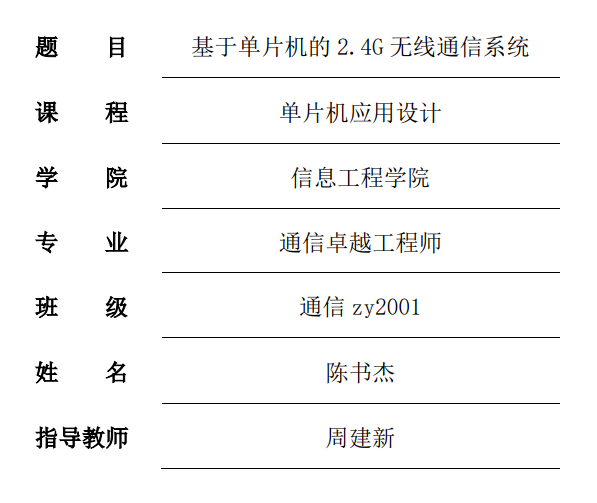
\includegraphics[scale=0.9]{2.png}
\end{figure} 
\thispagestyle{empty}
\clearpage

\centerline{\LARGE\textbf{《单片机应用设计》任务书}}
\begin{center}
\large{
\textbf{学生姓名:}\underline{陈书杰}\quad\textbf{专业班级:}\underline{通信zy2001}

\textbf{指导老师:}\underline{周建新}\quad\textbf{工作单位:}\underline{信息工程学院}

\textbf{题目:基于单片机的2.4G无线通信系统}
}
\end{center}
~\\
\large{\textbf{课程设计目的:}}\normalsize

1、熟悉单片机应用系统的硬件设计及软件设计的基本方法;

2、	将《单片机原理与应用》理论课的理论知识应用于实际的应用系统中;

3、	训练单片机应用技术,锻炼实际动手能力;

4、	提高正确地撰写论文的基本能力。

~\\
\large{\textbf{课程设计内容与要求:}}\normalsize

1、	完成硬件电路的设计,其中包括单片机和NRF24L01芯片模块的设计;
 
2、	完成无线通信模块的程序设计与实现,上机运行调试程序,记录实验结果(如图表等),并对实验结果进行分析和总结; 

3、	 课程设计报告书按学校统一规范来撰写,报告主要包括以下内容:目录、摘要、关键词、基本原理、方案论证、硬件设计、软件设计(带流程图、程序清单)、仿真结果、实物运行结果照片、结论献等;

4、	查阅不少于6篇参考文献。

~\\
\large{\textbf{初始条件:}}\normalsize

1、	STC89C52和NRF24L01模块; 

2、	先修课程:单片机原理与应用。

~\\
\large{\textbf{时间安排:}}\normalsize

第17周,安排设计任务,完成硬件设计;

第18周,完成软件设计、撰写报告,答辩。

~\\
\large\textbf{指导老师签名:\hfill 年\quad\quad 月\quad\quad 日}

~\\
\large\textbf{系主任(或责任教师)签名:\hfill 年\quad\quad 月\quad\quad 日}\normalsize
\thispagestyle{empty}
\clearpage

\tableofcontents
\thispagestyle{empty}
\clearpage

\setcounter{page}{1}
\section*{摘要}
\addcontentsline{toc}{section}{摘要}
本次设计的任务目标为使用NRF24L01芯片构成无线传输模块,实现2.4G无线通信系统的构建。设计采用了以STM32f103为主控芯片的单片机开发平台,通过串行外设接口控制NRF24L01,在电脑端利用串口调试助手,实现了芯片配置以及数据传输。经不断调试,本此设计的系统最终成功实现了所有指标。

{\large\textbf{关键字:}}2.4G无线通信;STM32开发;NRF24L01;串口调试
\clearpage

\section*{Abstract}
\addcontentsline{toc}{section}{Abstract}
The task goal of this design is to use NRF24L01 chip to construct wireless transmission module to build  2.4G wireless transmission system. The design adopts a single-chip microcomputer development platform with STM32f103 as the main control chip, which controls the NRF24L01 through the serial peripheral interface. We use the serial port debugging assistant on the computer side to realize chip configuration and data transmission. After continuous debugging, the system of this design was finally successfully achieved all indicators.

{\large\textbf{Key Words:}}2.4G Wireless Transmission; STM32 development; NRF24L01; Serial Port Debugging Assistant
\clearpage

\section{基本原理}
\subsection{无线通讯技术}
无线通信是利用电磁波信号可以在自由空间中传播的特性进行信息交换的一种通信方式,近些年信息通信领域中,发展最快、应用最广的就是无线通信技术。在移动中实现的无线通信又通称为移动通信,人们把二者合称为无线移动通信。

无线通信主要包括微波通信和卫星通信。微波是一种无线电波,它传送的距离一般只有几十千米。但微波的频带很宽,通信容量很大。微波通信每隔几十千米要建一个微波中继站。卫星通信是利用通信卫星作为中继站在地面上两个或多个地球站之间或移动体之间建立微波通信联系。
 
\subsection{2.4GHz无线技术}
2.4GHz是物联网前端接入通讯所采用的重要频段。由国际组织推动的Wi-Fi、蓝牙和ZigBee技术,以及大量各厂商自行开发的技术方案,都支持工作在这一频段之上。

要说明2.4G技术,还要先从ISM频段谈起。ISM频段是国际电信联盟规定的保留频段,用于工业(industry)、科学研究(science)以及微波医疗(medical)方面的应用,最初并未打算大规模用于数据通讯。1947年亚特兰大的国际通讯大会上,美国代表团首先提出了希望设立ISM频段的要求,此后ISM频段逐渐被各国承认。

近年来,ISM频段也开始被免许可和容错通讯设备所采用,像无线传感网络、无线本地网络和无绳电话等,越来越多消费电子产品在无线通讯中采用ISM频段。如图1,某品牌蓝牙鼠标使用的就是属于ISM频段的2.4G通信系统。

\begin{figure}[htbp]
    \centering
    
\includegraphics[scale=0.4]{mouse.jpg}
    \caption{某品牌鼠标的宣传广告}
\end{figure} 

433MHz和2.4GHz都是ISM频段的一员,但ISM频段在各国中的规定并不相同,2.4GHz 频段是比433MHz频段更广泛的、各国共同承认和遵守的ISM频段,蓝牙、Wi-Fi、ZigBee 等通讯协议和标准,都明确支持工作在2.4GHz频段。

由于2.4GHz频段有着众多优势,包括蓝牙、ZigBee、Wi-Fi等众多技术都支持工作在这一频段之上,并通过协议和标准的更新完善提供了众多亮点功能,比如Mesh组网、直接联网等。2016年,ZigBee 3.0标准发布,增强支持直接联网(Direct Internet Connections),且此前已经实现了Mesh自组网。Mesh和IP通讯能力,对于物联网应用来说都是非常重要的。

受政策利好和行业发展影响,2.4G技术在物联网的应用被普遍看好。其中基于2.4GHz 频段的私有协议技术灵活性更高,能够实现更具个性化、适用于各种应用场景的物联网应用。
\clearpage

\section{系统设计方案}
\subsection{无线通信模块方案选择}
\subsubsection{NRF24L01}
NRF24L01是一款工作在2.4-2.5GHz世界通用ISM频段的单片无线收发器芯片。无线收发器包括:频率发生器、增强型SchockBurst模式控制器、功率放大器、晶体振荡器、调制器、解调器。输出功率、频道选择和协议的设置可以通过SPI接口进行设置。其芯片结构如图2所示。

\begin{figure}[htbp]
    \centering
    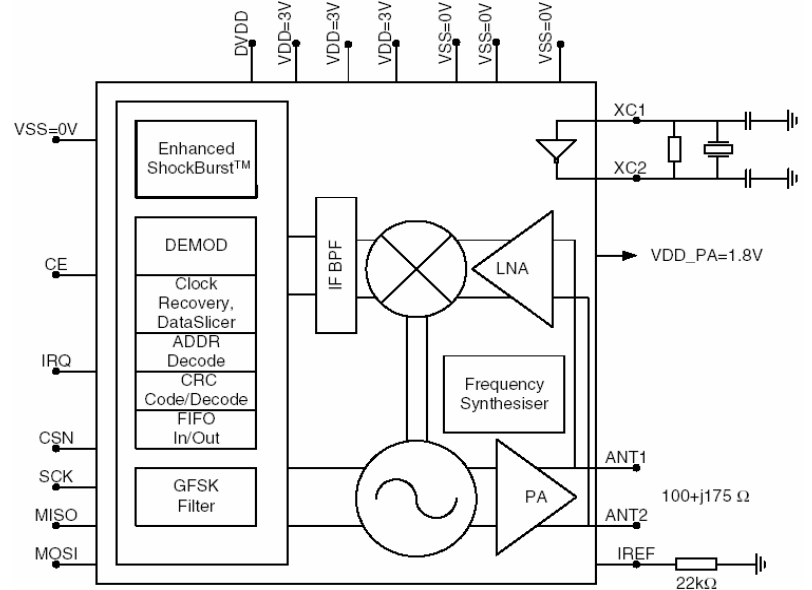
\includegraphics[scale=0.6]{p1.png}
    \caption{NRF24L01芯片结构}
\end{figure} 

极低的电流消耗:当工作在发射模式下发射功率为-6dBm时电流消耗为9mA,接收模式时为12.3mA。掉电模式和待机模式下电流消耗更低。

而Telesky公司以NRF24L01芯片为核心,开发了一款商用级的2.4G通信模块,它有8个间距0.1英寸的引脚,如图3所示。

\begin{figure}[htbp]
    \centering
    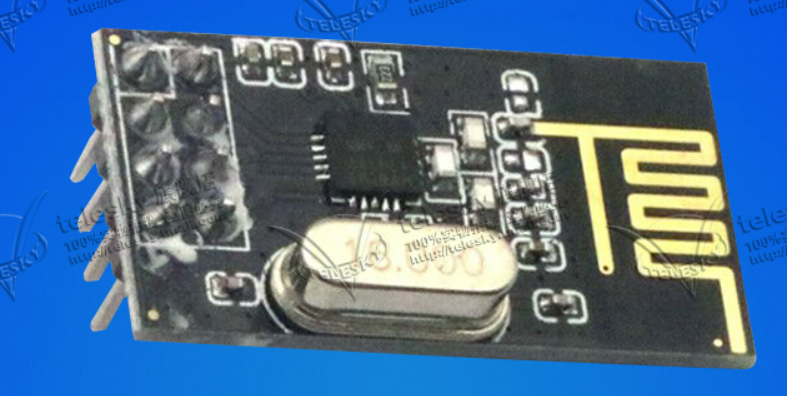
\includegraphics[scale=0.6]{p2.png}
    \caption{Telesky公司2.4G通信产品}
\end{figure} 

此模块的PCB设计图如图4所示。
\begin{figure}[htbp]
    \centering
    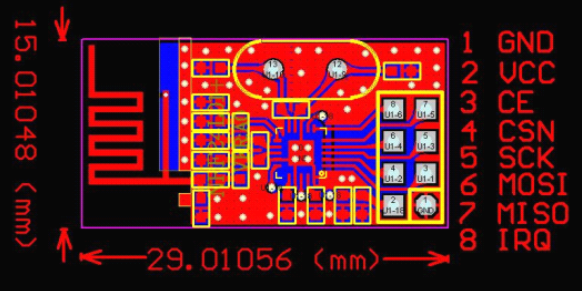
\includegraphics[scale=0.8]{p3.png}
    \caption{此产品的PCB设计图}
\end{figure} 

VCC脚接电压范围为1.9V-3.6V之间,不能在这个区间之外,超过3.6V将会烧毁模块。推荐电3.3V左右。除电源VCC和接地端,其余脚都可以直接和普通的5V单片机IO口直接相连,无需电平转换。当然对3V左右的单片机更加适用了。硬件上面没有SPI的单片机也可以控制本模块,用普通单片机IO口模拟SPI不需要单片机真正的串口介入,只需要普通的单片机IO口就可以了,当然用串口也可以了。

除了VCC和GND以外,此模块还有6个控制与数据管脚,它们的功能如下:
\begin{itemize}
\item CSN:芯片的片选线,CSN为低电平芯片工作
\item SCK:芯片控制的时钟线(SPI时钟)
\item MISO:芯片控制数据线(Master input slave output)
\item MOSI:芯片控制数据线(Master output slave input)
\item IRQ:中断信号,无线通信过程中MCU主要是通过IRQ与NRF24L01进行通信
\item CE:芯片的模式控制线,在CSN为低的情况下,CE协同NRF24L01的CONFIG寄存器共同决定NRF24L01的状态
\end{itemize}

NRF24L01共有5种模式:
\begin{itemize}
\item Power Down Mode:掉电模式
\item Tx Mode:发射模式
\item Rx Mode:接收模式
\item Standby-1 Mode:待机1模式
\item Standby-2 Mode:待机2模式
\end{itemize}

图5显示了模块在不同状态下引脚的功能

\begin{figure}[htbp]
    \centering
    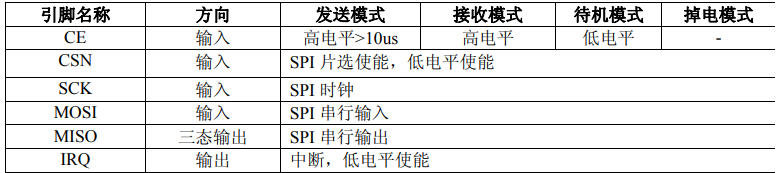
\includegraphics[scale=0.8]{p4.png}
    \caption{NRF24L01引脚功能}
\end{figure} 

\subsubsection{CC2500}
CC2500无线模块是美国TI的产品(如图6),与NRF24L01相比,具有OOK/ASK/2-FSK/MSK等多种调制方式,在不同的环境中可以根据需要采取相应的工作方式,提高了工作效率。CC2500的输出功率比NRF24L01高,最高可达1dbm;支持每个数据包连接质量指示;具有单独的 64 字节RX和TX数据 FIFO,能依次发送或者接收更大的数据包;在芯片中集成了各种纠错评估指示电路,属于一种比较严谨的数传模块。它的不足之处在于传输速率不如NRF24L01。

\begin{figure}[htbp]
    \centering
    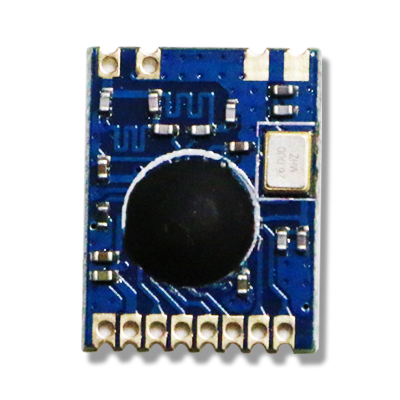
\includegraphics[scale=0.8]{p5.png}
    \caption{CC2500外观}
\end{figure} 

由于CC2500结构较为复杂,工程量较NRF24L01会多很多。本报告作为探究实验类报告,不需要高强度商业用芯片进行实验,因此选NRF24L01作为主控模块。

\subsection{主控单片机方案选择}
\subsubsection{STC89C52}
STC89C52是51单片机的一个型号,51单片机是对兼容英特尔8051指令系统的单片机的统称。51单片机广泛应用于家用电器、汽车、工业测控、通信设备中。因为51单片机的指令系统、内部结构相对简单,所以国内许多高校用其进行单片机入门教学。STC89C52模块的核心如图7所示。

\begin{figure}[htbp]
    \centering
    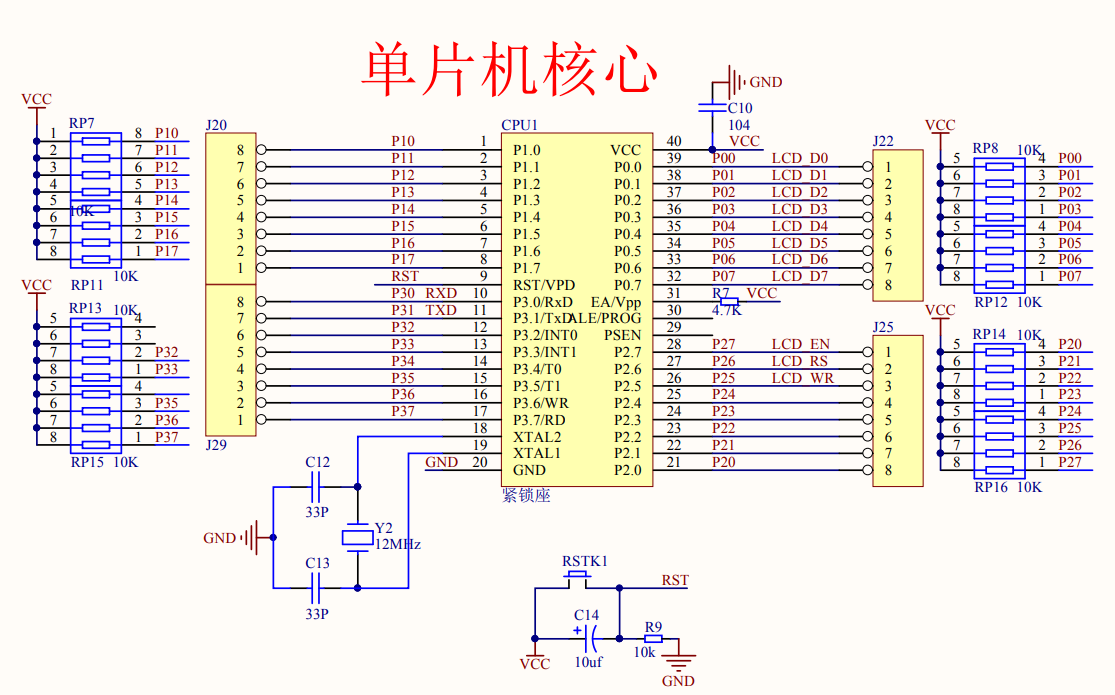
\includegraphics[scale=0.6]{p6.png}
    \caption{某型号51单片机开发板核心}
\end{figure} 

\subsubsection{STM32f103}
进入21世纪,市场产品竞争越来越激烈,对成本极其敏感,相应地对 MCU 的性能要求也更苛刻:更多功能,更低功耗,易用界面和多任务。基于这样的市场需求,ARM 公司推出了其全新的基于 ARMv7 架构的 32 位 Cortex-M3 微控制器内核。紧随其后,ST(意法半导体)公司就推出了基于 Cortex-M3 内核的 MCU—STM32。STM32,凭借其产品线的多样化、极高的性价比、简单易用的库开发方式,迅速在众多 Cortex-M3 MCU 中脱颖而出,成为最闪亮的一颗新星。STM32 一上市就迅速占领了中低端 MCU 市场,受到了市场和工程师的无比青睐,颇有星火燎原之势。某型号的STM32单片机核心如图8所示。

野火公司依托意法半导体的芯片,研制出了一系列STM32单片机开发板。野火公司会为它设计的每款开发板配套图书、教学视频和例程。初学者可以通过这些资料快速入门,掌握嵌入式开发的技能。

STC89C52虽然是一款实用的单片机,但是它已经很古老了。8051指令系统是1979年诞生的,距今已经四十余年。它的硬件资源和更加先进的处理器相比已经比较落后了。而且,STM32由于火热异常,它的相关资料一般会更多,所以,我们这次设计选择STM32f103 作为主控单片机。

\begin{figure}[htbp]
    \centering
    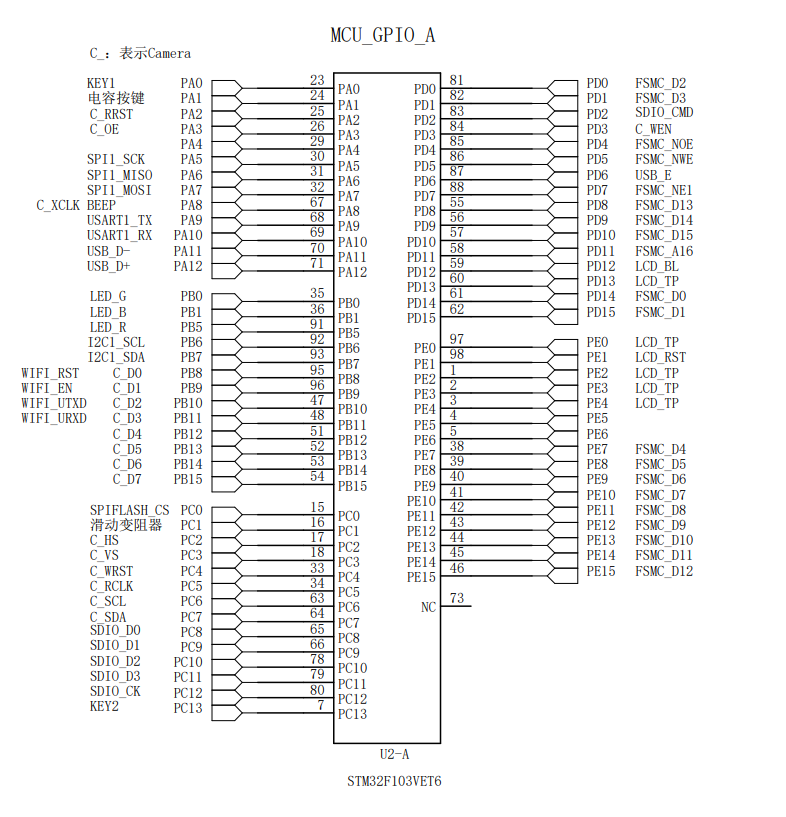
\includegraphics[scale=0.9]{p7.png}
    \caption{某型号STM32单片机开发板核心}
\end{figure} 

\subsection{系统构成框图}
本设计的系统构成框图如图9所示。可以看出,我要设计的是一个对称的结构,每一端既可以作为接收方,也可以作为发送方。数据首先从发送端的串口调试助手发出,经过发送端的单片机送进发送端的NRF24L01中。两片NRF24L01之间进行无线通信,接收端的NRF24L01收到数据后,经单片机送入接收端的串口调试助手。这样一整个通信流程就结束了。
\begin{figure}[htbp]
    \centering
    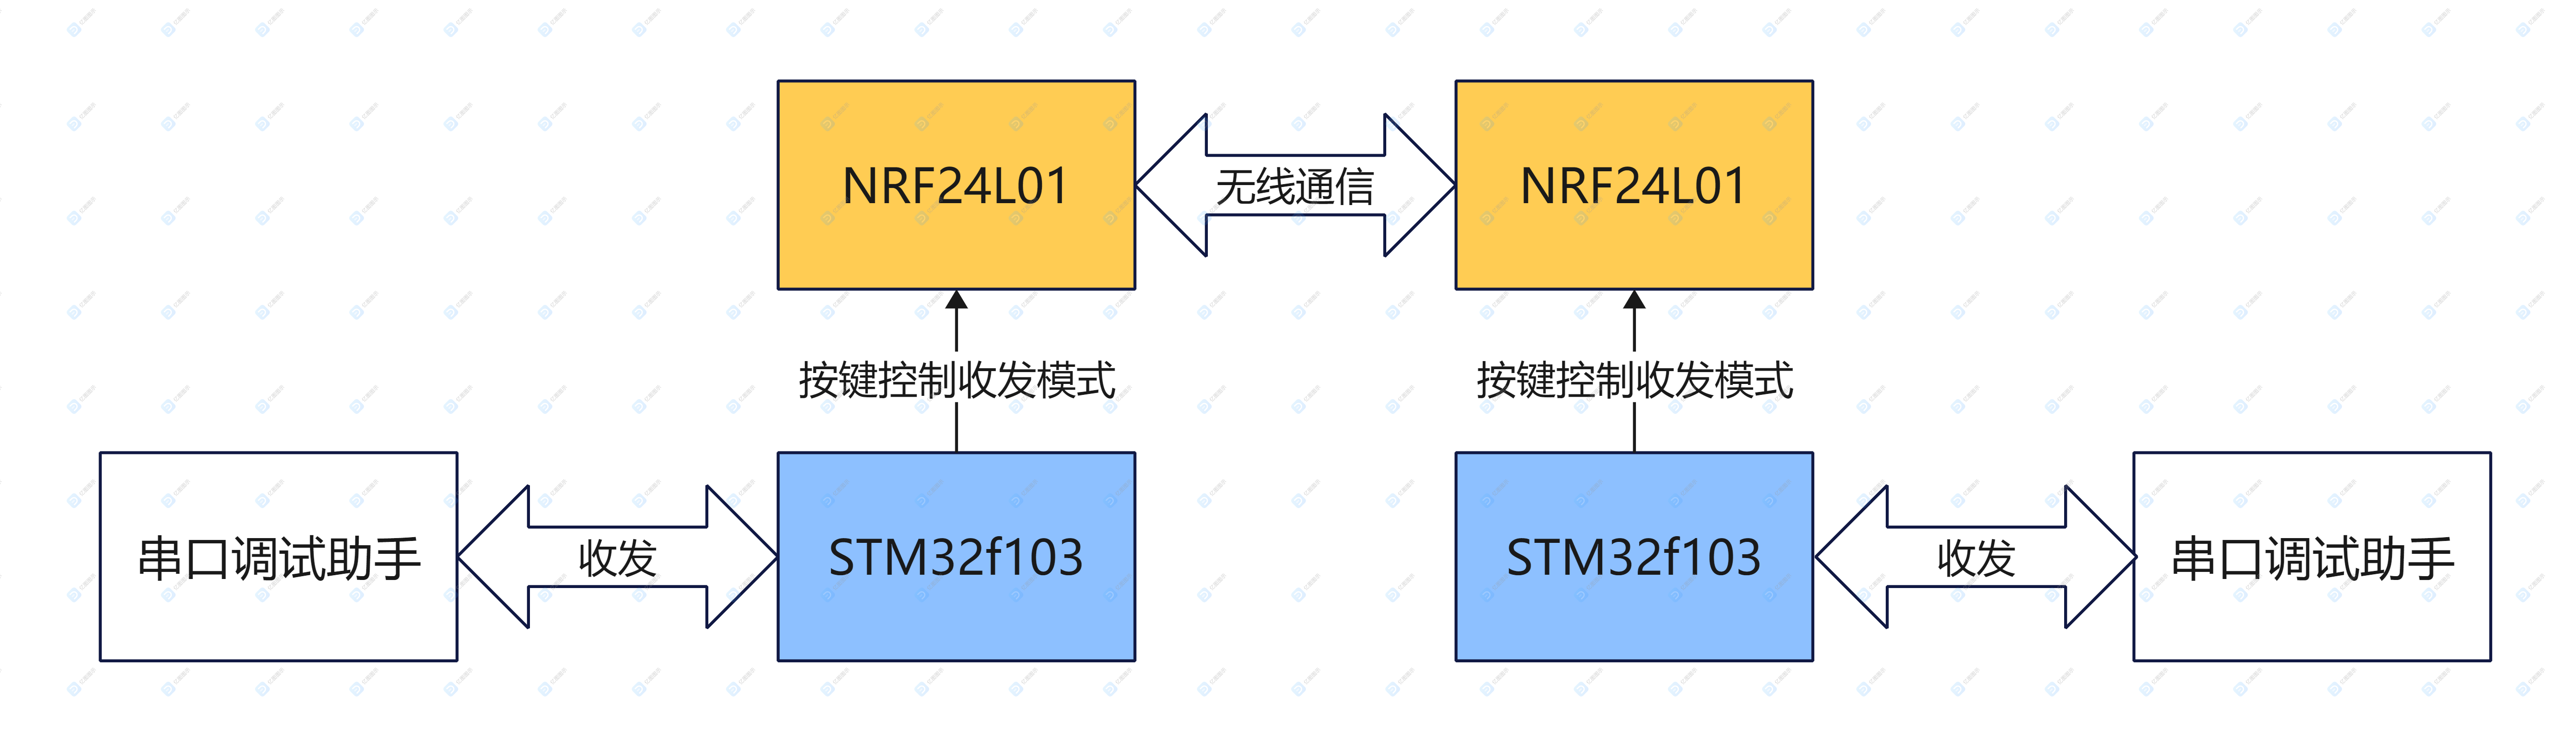
\includegraphics[scale=0.1]{p8.png}
    \caption{系统构成框图}
\end{figure} 
\clearpage

\section{系统硬件设计}
\subsection{单片机与通信模块的连接}
这次的设计我用的是基于STM32f103vet6的野火指南者开发板,如图10所示,红圈处有一个2*4的排母,是专门设计用来和NRF24L01适配的,如图11。

\begin{figure}[htbp]
    \centering
    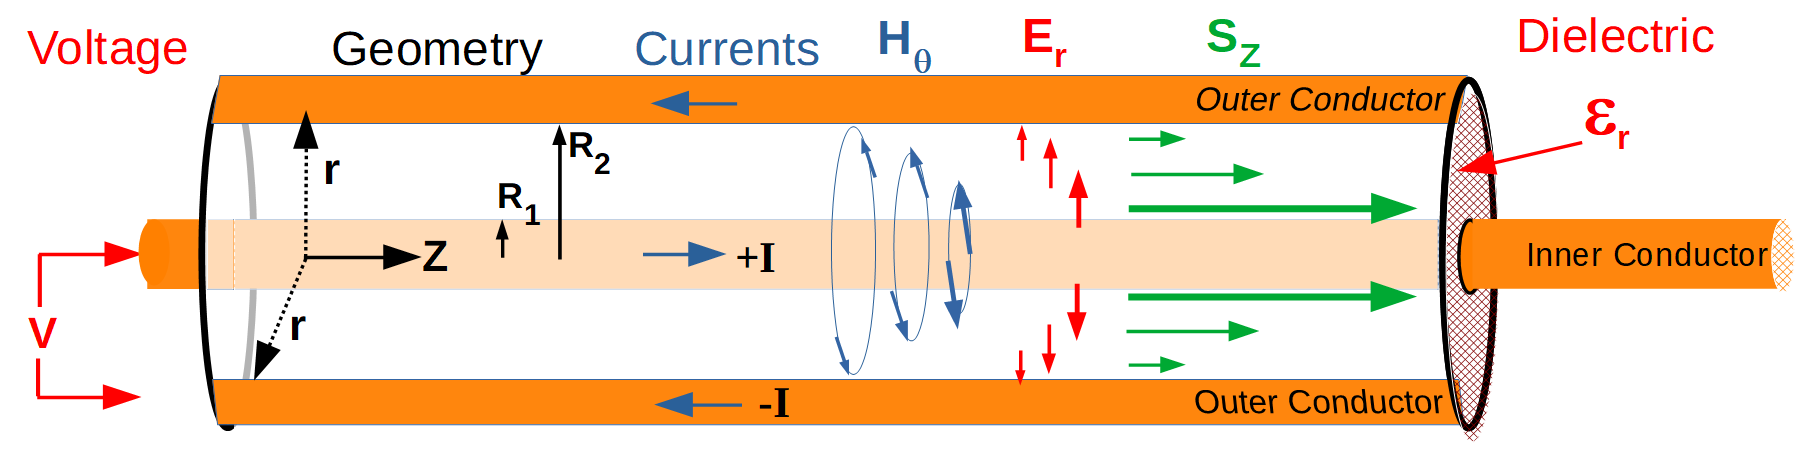
\includegraphics[scale=0.06]{p10.jpg}
    \caption{指南者开发板}
\end{figure} 

\begin{figure}[htbp]
    \centering
    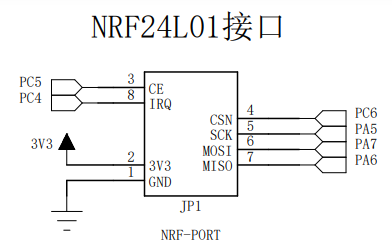
\includegraphics{p11.png}
    \caption{开发板上的NRF24L01接口}
\end{figure} 

\subsection{机械按钮}
在开发过程中,我们会使用到按钮k1。按键机械触点断开、闭合时,由于触点的弹性作用,按键开关不会马上稳定接通或一下子断开,使用按键时会产生波纹信号,需要用软件消抖处理滤波,不方便输入检测。而指南者连接的按键带硬件消抖功能,见图按键原理图 ,它利用电容充放电的延时,消除了波纹,从而简化软件的处理,软件只需要直接检测引脚的电平即可。

从图12可知,这些按键在没有被按下的时候,GPIO 引脚的输入状态为低电平 (按键所在的电路不通,引脚接地),当按键按下时,GPIO 引脚的输入状态为高电平 (按键所在的电路导通,引脚接到电源)。只要我们检测引脚的输入电平,即可判断按键是否被按下。

\begin{figure}[htbp]
    \centering
    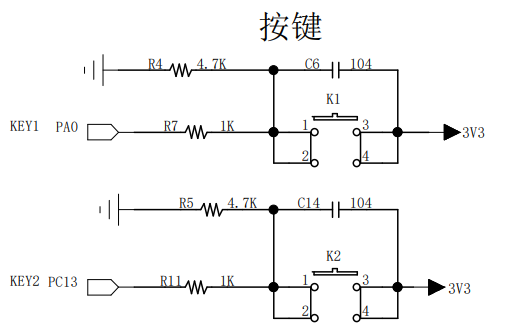
\includegraphics{p12.png}
    \caption{开发板上的机械按键}
\end{figure} 
\clearpage

\section{系统软件设计}
\subsection{按键配置程序}
我们使用STM32的标准库进行编程,对按键K1的配置流程图如下:
\begin{figure}[htbp]
    \centering
    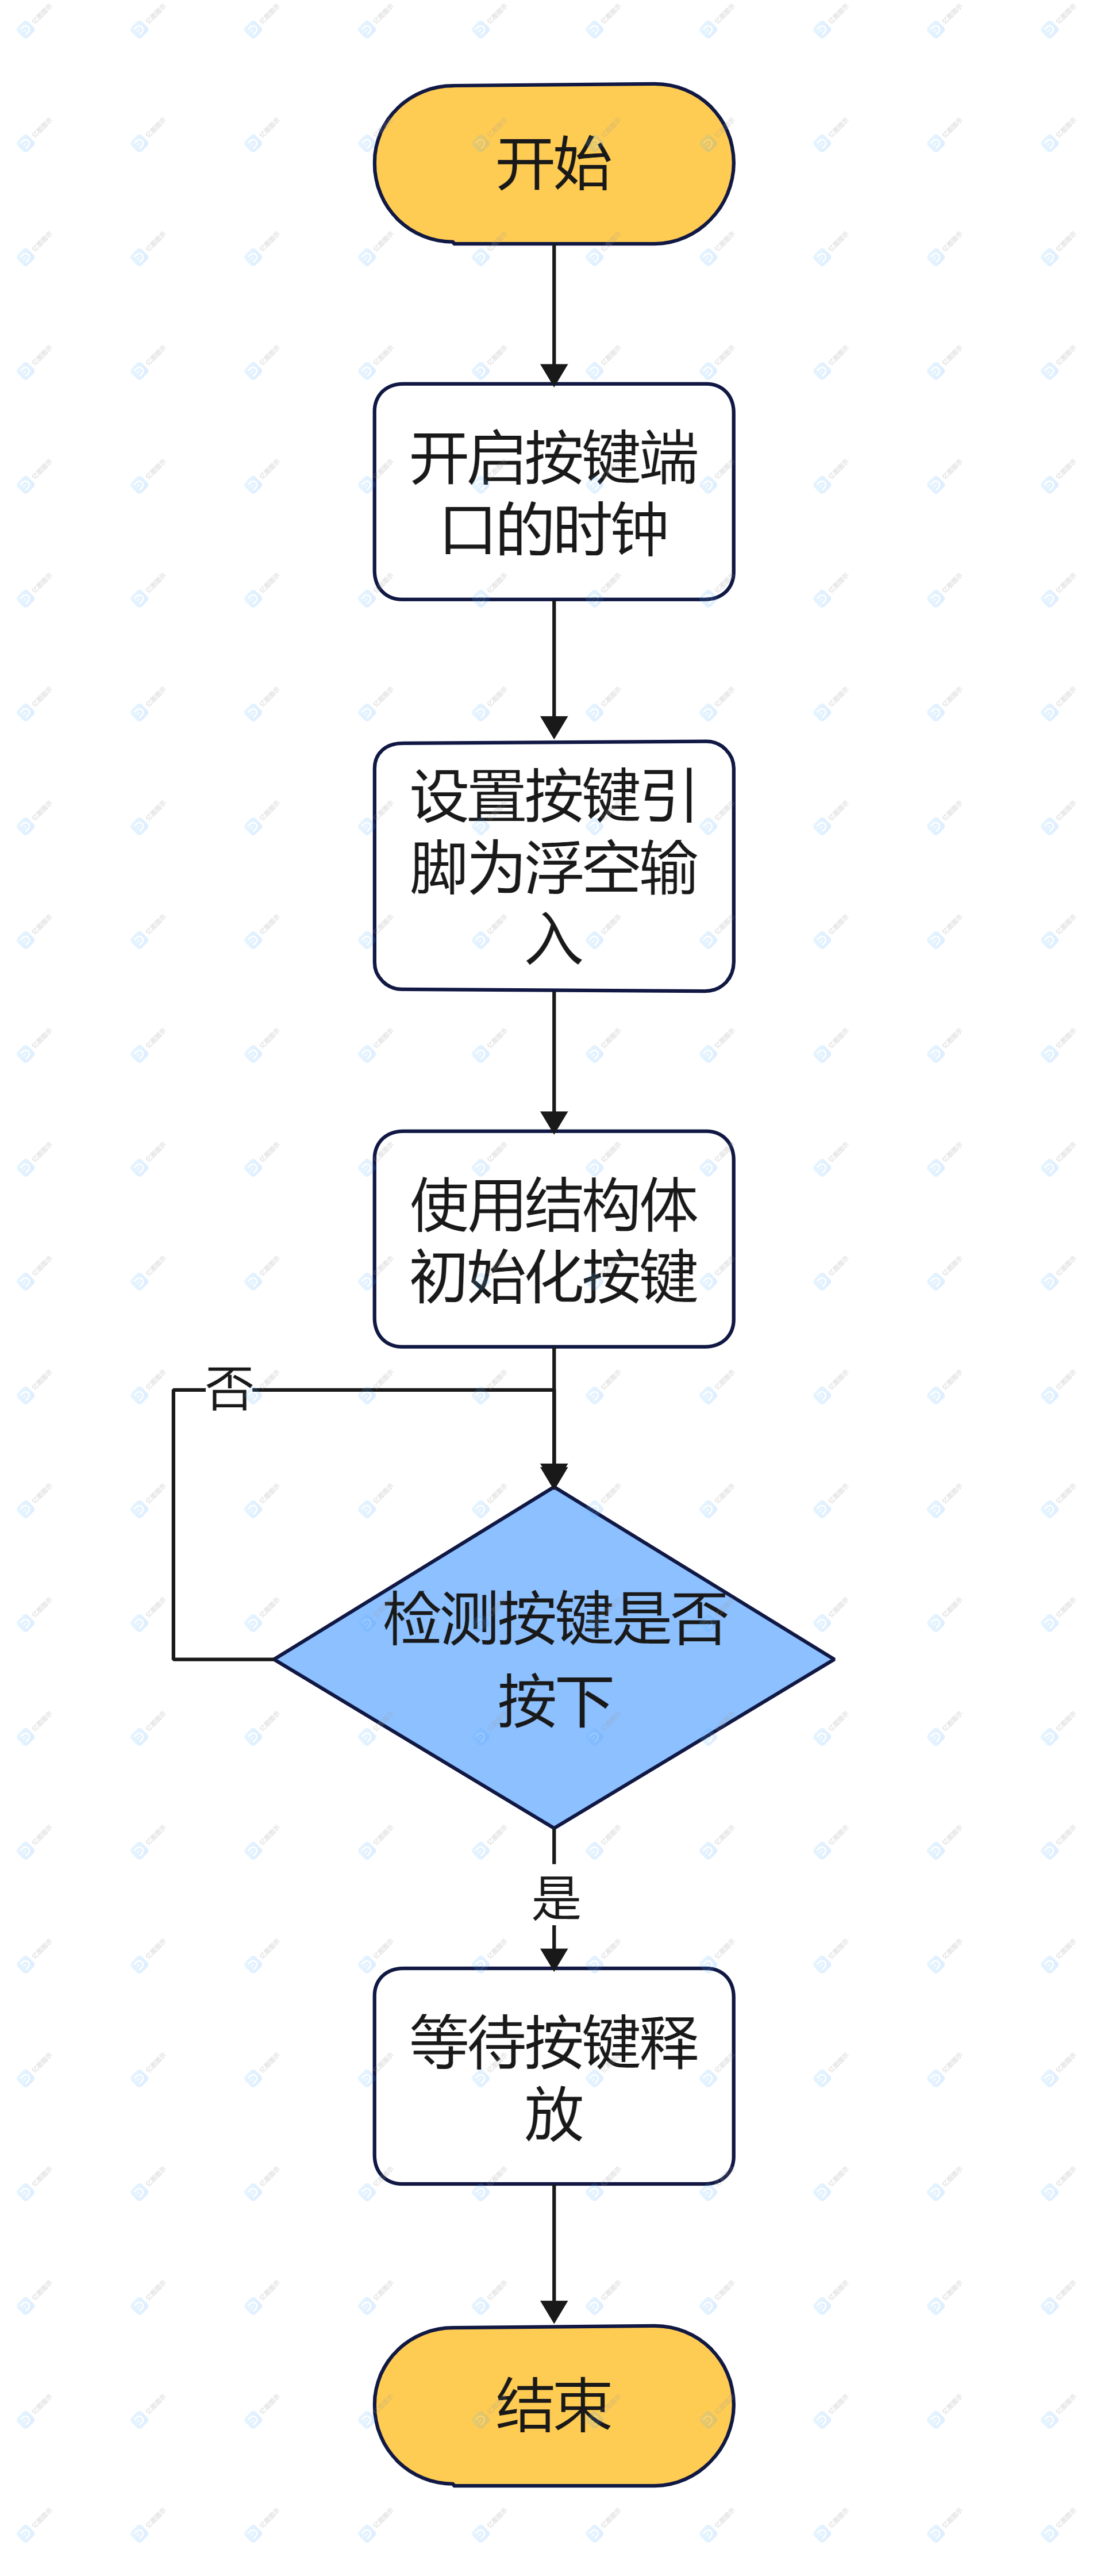
\includegraphics[scale=0.15]{p13.png}
    \caption{按键配置流程图}
\end{figure} 

所以我们可以编写如下的程序,使得按键K1可以成为设计的一部分。
\begin{lstlisting}[caption={}]
#include "./key/bsp_key.h"  

void Key_GPIO_Config(void)
{
	GPIO_InitTypeDef GPIO_InitStructure;
	
	/*开启按键端口的时钟*/
	RCC_APB2PeriphClockCmd(KEY1_GPIO_CLK|KEY2_GPIO_CLK,ENABLE);
	
	//选择按键的引脚
	GPIO_InitStructure.GPIO_Pin = KEY1_GPIO_PIN; 
	// 设置按键的引脚为浮空输入
	GPIO_InitStructure.GPIO_Mode = GPIO_Mode_IN_FLOATING; 
	//使用结构体初始化按键
	GPIO_Init(KEY1_GPIO_PORT, &GPIO_InitStructure);
	
	//选择按键的引脚
	GPIO_InitStructure.GPIO_Pin = KEY2_GPIO_PIN; 
	//设置按键的引脚为浮空输入
	GPIO_InitStructure.GPIO_Mode = GPIO_Mode_IN_FLOATING; 
	//使用结构体初始化按键
	GPIO_Init(KEY2_GPIO_PORT, &GPIO_InitStructure);	
}

uint8_t Key_Scan(GPIO_TypeDef* GPIOx,uint16_t GPIO_Pin)
{			
	/*检测是否有按键按下 */
	if(GPIO_ReadInputDataBit(GPIOx,GPIO_Pin) == KEY_ON )  
	{	 
		/*等待按键释放 */
		while(GPIO_ReadInputDataBit(GPIOx,GPIO_Pin) == KEY_ON);   
		return 	KEY_ON;	 
	}
	else
		return KEY_OFF;
}
\end{lstlisting}

\subsection{串口通信配置程序}
串口通讯 (Serial Communication)是一种设备间非常常用的串行通讯方式,因为它简单便捷,因此大部分电子设备都支持该通讯方式,电子工程师在调试设备时也经常使用该通讯方式输出调试信息。

通用同步异步收发器 (Universal Synchronous Asynchronous Receiver and Transmitter)是一个串行通
信设备,可以灵活地与外部设备进行全双工数据交换。有别于 USART 还有一个 UART(Universal
Asynchronous Receiver and Transmitter),它是在 USART 基础上裁剪掉了同步通信功能,只有异步
通信。简单区分同步和异步就是看通信时需不需要对外提供时钟输出,我们平时用的串口通信基
本都是 UART。USART的结构如图14所示。

\begin{figure}[htbp]
    \centering
    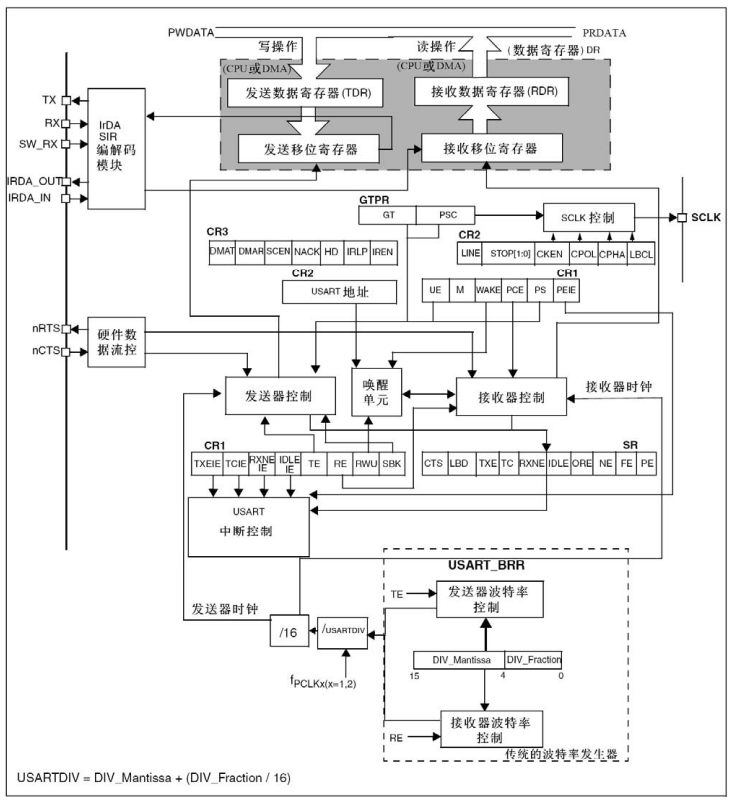
\includegraphics[scale=0.9]{p14.png}
    \caption{USART结构}
\end{figure} 

STM32f103vet6 系统控制器有三个 USART 和两个 UART(其引脚分布如图15),其中 USART1 和时钟来源于 APB2 总线时钟,其最大频率为 72MHz,其他四个的时钟来源于 APB1 总线时钟,其最大频率为 36MHz。UART 只是异步传输功能,所以没有 SCLK、nCTS 和 nRTS 功能引脚。

\begin{figure}[htbp]
    \centering
    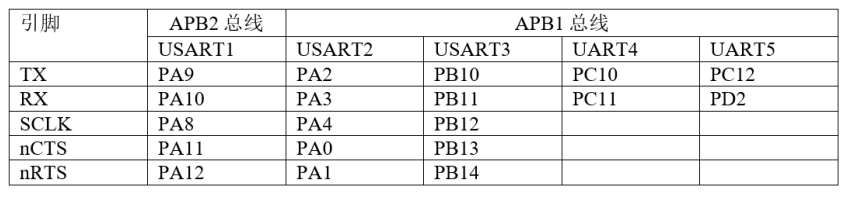
\includegraphics[scale=0.7]{p15.png}
    \caption{USART引脚分布}
\end{figure}

USART 数据寄存器只有低 9 位有效,并且第 9 位数据是否有效要取决于 USART控制寄存器 1的 M 位设置,当 M 位为 0 时表示 8 位数据字长,当 M 位为 1 表示 9位数据字长,我们一般使用 8 位数据字长。

波特率指数据信号对载波的调制速率,它用单位时间内载波调制状态改变次数来表示,单位为波
特。比特率指单位时间内传输的比特数,单位 bit/s(bps)。对于 USART 波特率与比特率相等,以
后不区分这两个概念。波特率越大,传输速率越快。

综上所述,我们可以画出串口通信的配置流程图。

\begin{figure}[htbp]
    \centering
    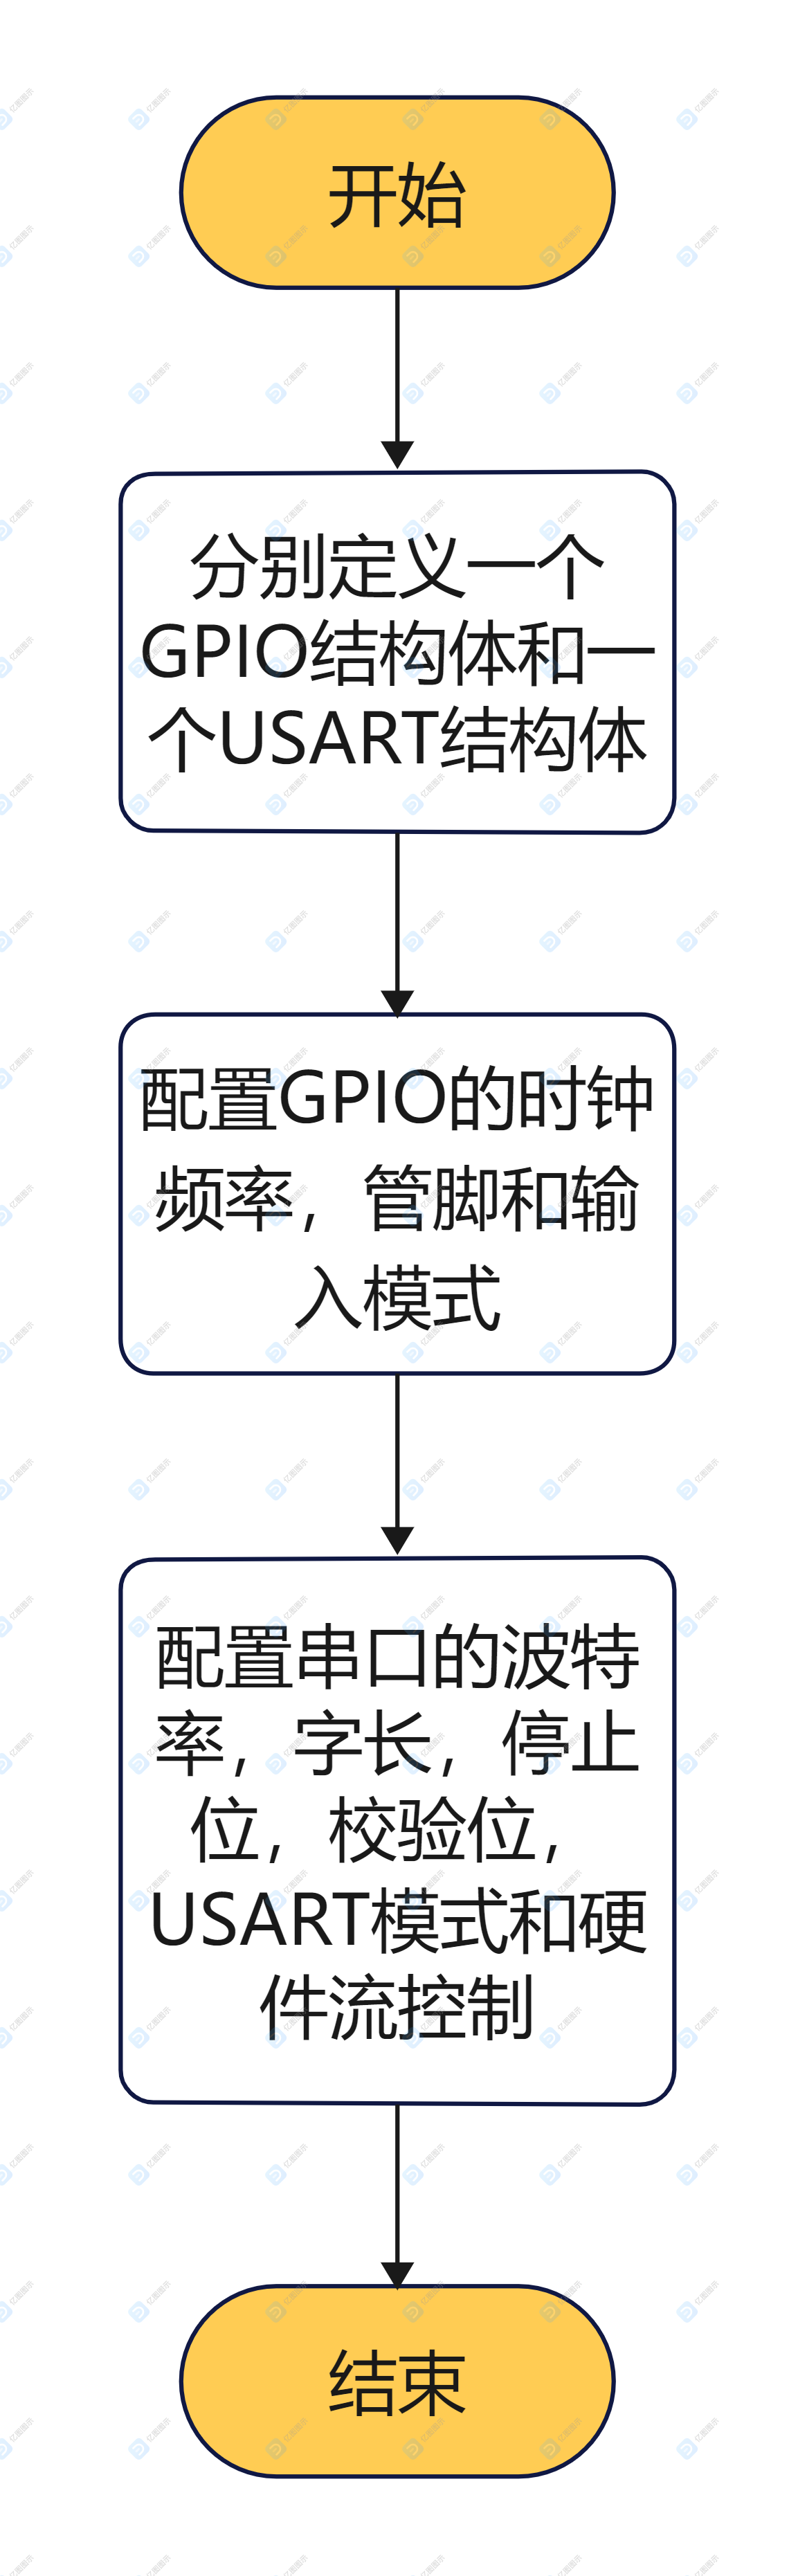
\includegraphics[scale=0.14]{p16.png}
    \caption{串口通信配置流程图}
\end{figure} 

我们可以编写出如下的配置代码。

\begin{lstlisting}[caption={}]
#include "bsp_usart1.h"

void USART1_Config(void)
{
	GPIO_InitTypeDef GPIO_InitStructure;
	USART_InitTypeDef USART_InitStructure;
		
	/* config USART1 clock */
	RCC_APB2PeriphClockCmd(RCC_APB2Periph_USART1 | RCC_APB2Periph_GPIOA, ENABLE);
		
	/* USART1 GPIO config */
	/* Configure USART1 Tx (PA.09) as alternate function push-pull */
	GPIO_InitStructure.GPIO_Pin = GPIO_Pin_9;
	GPIO_InitStructure.GPIO_Mode = GPIO_Mode_AF_PP;
	GPIO_InitStructure.GPIO_Speed = GPIO_Speed_50MHz;
	GPIO_Init(GPIOA, &GPIO_InitStructure);    
	/* Configure USART1 Rx (PA.10) as input floating */
	GPIO_InitStructure.GPIO_Pin = GPIO_Pin_10;
	GPIO_InitStructure.GPIO_Mode = GPIO_Mode_IN_FLOATING;
	GPIO_Init(GPIOA, &GPIO_InitStructure);
			
	/* USART1 mode config */
	USART_InitStructure.USART_BaudRate = 115200;
	USART_InitStructure.USART_WordLength = USART_WordLength_8b;
	USART_InitStructure.USART_StopBits = USART_StopBits_1;
	USART_InitStructure.USART_Parity = USART_Parity_No ;
	USART_InitStructure.USART_HardwareFlowControl = USART_HardwareFlowControl_None;
	USART_InitStructure.USART_Mode = USART_Mode_Rx | USART_Mode_Tx;
	USART_Init(USART1, &USART_InitStructure); 
	USART_Cmd(USART1, ENABLE);
}

int fputc(int ch, FILE *f)
{
	/* 发送一个字节数据到USART1 */
	USART_SendData(USART1, (uint8_t) ch);
		
	/* 等待发送完毕 */
	while (USART_GetFlagStatus(USART1, USART_FLAG_TXE) == RESET);		
	
	return (ch);
}

int fgetc(FILE *f)
{
	/* 等待串口1输入数据 */
	while (USART_GetFlagStatus(USART1, USART_FLAG_RXNE) == RESET);

	return (int)USART_ReceiveData(USART1);
}
\end{lstlisting}

由程序可知,我们设置的波特率是115200。字长为8,一位停止位,无校验位。第33行开始,我们编写了两个重定向函数,把C语言的 fputc 和 fgetc 函数赋予了读写串口的功能。

\subsection{NRF24L01配置程序}
通过上一章的知识,我们可以编写出无线通信模块的配置程序。(由于程序较为复杂,此处暂不画流程图)

\begin{lstlisting}[caption={}]
#include "bsp_spi_nrf.h"
#include "bsp_usart1.h"

u8 RX_BUF[RX_PLOAD_WIDTH];		//接收数据缓存
u8 TX_BUF[TX_PLOAD_WIDTH];		//发射数据缓存
u8 TX_ADDRESS[TX_ADR_WIDTH] = {0x34,0x43,0x10,0x10,0x01};  
	// 定义一个静态发送地址
u8 RX_ADDRESS[RX_ADR_WIDTH] = {0x34,0x43,0x10,0x10,0x01}; 

void Delay(__IO u32 nCount)
{
  	for(; nCount != 0; nCount--);
} 

void SPI_NRF_Init(void)  
{
	SPI_InitTypeDef  SPI_InitStructure;
  	GPIO_InitTypeDef GPIO_InitStructure;
  
  	RCC_APB2PeriphClockCmd(RCC_APB2Periph_GPIOA
                 	|NRF_IRQ_GPIO_CLK
                   	|NRF_CSN_GPIO_CLK
                    	|NRF_CE_GPIO_CLK,ENABLE);

  	RCC_APB2PeriphClockCmd(RCC_APB2Periph_SPI1, ENABLE);

  	GPIO_InitStructure.GPIO_Pin = GPIO_Pin_5|GPIO_Pin_6|GPIO_Pin_7;
  	GPIO_InitStructure.GPIO_Speed = GPIO_Speed_10MHz;
  	GPIO_InitStructure.GPIO_Mode = GPIO_Mode_AF_PP; //复用功能
  	GPIO_Init(GPIOA, &GPIO_InitStructure);  

  	GPIO_InitStructure.GPIO_Pin = NRF_CSN_PIN;
  	GPIO_InitStructure.GPIO_Speed = GPIO_Speed_10MHz;
  	GPIO_InitStructure.GPIO_Mode = GPIO_Mode_Out_PP;
  	GPIO_Init(NRF_CSN_GPIO_PORT, &GPIO_InitStructure);
  
  	GPIO_InitStructure.GPIO_Pin = NRF_CE_PIN;
  	GPIO_InitStructure.GPIO_Speed = GPIO_Speed_10MHz;
  	GPIO_InitStructure.GPIO_Mode = GPIO_Mode_Out_PP;
  	GPIO_Init(NRF_CE_GPIO_PORT, &GPIO_InitStructure);
  
  	GPIO_InitStructure.GPIO_Pin = NRF_IRQ_PIN;
  	GPIO_InitStructure.GPIO_Speed = GPIO_Speed_10MHz;
  	GPIO_InitStructure.GPIO_Mode = GPIO_Mode_IPU ;  //上拉输入
  	GPIO_Init(NRF_IRQ_GPIO_PORT, &GPIO_InitStructure); 
		  
  	NRF_CSN_HIGH(); 
 
  	SPI_InitStructure.SPI_Direction = SPI_Direction_2Lines_FullDuplex; 
	//双线全双工
  	SPI_InitStructure.SPI_Mode = SPI_Mode_Master;	 				//主模式
  	SPI_InitStructure.SPI_DataSize = SPI_DataSize_8b;	 				
  	SPI_InitStructure.SPI_CPOL = SPI_CPOL_Low;		 	//时钟极性,空闲时为低
  	SPI_InitStructure.SPI_CPHA = SPI_CPHA_1Edge;	
  	SPI_InitStructure.SPI_NSS = SPI_NSS_Soft;		   					
  	SPI_InitStructure.SPI_BaudRatePrescaler = SPI_BaudRatePrescaler_8;  
  	SPI_InitStructure.SPI_FirstBit = SPI_FirstBit_MSB;  				//高位在前
  	SPI_InitStructure.SPI_CRCPolynomial = 7;
  	SPI_Init(SPI1, &SPI_InitStructure);

  	/* Enable SPI1  */
  	SPI_Cmd(SPI1, ENABLE);
}

u8 SPI_NRF_RW(u8 dat)  
{  	
	while (SPI_I2S_GetFlagStatus(SPI1, SPI_I2S_FLAG_TXE) == RESET);

	SPI_I2S_SendData(SPI1, dat);		

	while (SPI_I2S_GetFlagStatus(SPI1, SPI_I2S_FLAG_RXNE) == RESET);

	/* Return the byte read from the SPI bus */
	return SPI_I2S_ReceiveData(SPI1);
}


u8 SPI_NRF_WriteReg(u8 reg,u8 dat)  
{
 	u8 status;
	NRF_CE_LOW();
	NRF_CSN_LOW();

	/*发送命令及寄存器号 */
	status = SPI_NRF_RW(reg);

	/*向寄存器写入数据*/
	SPI_NRF_RW(dat);
	NRF_CSN_HIGH();	

	/*返回状态寄存器的值*/
	return(status);
}

u8 SPI_NRF_ReadReg(u8 reg)  
{
 	u8 reg_val;
	NRF_CE_LOW();
 	NRF_CSN_LOW();

  	/*发送寄存器号*/
	SPI_NRF_RW(reg);

	/*读取寄存器的值 */
	reg_val = SPI_NRF_RW(NOP);
	NRF_CSN_HIGH();		
	return reg_val;
}	

u8 SPI_NRF_ReadBuf(u8 reg,u8 *pBuf,u8 bytes)  
{
 	u8 status, byte_cnt;
	NRF_CE_LOW();
	NRF_CSN_LOW();

	/*发送寄存器号*/		
	status = SPI_NRF_RW(reg); 

 	/*读取缓冲区数据*/
	for(byte_cnt=0;byte_cnt<bytes;byte_cnt++)		  
	 	pBuf[byte_cnt] = SPI_NRF_RW(NOP); 
	NRF_CSN_HIGH();	
 	return status;		//返回寄存器状态值
}

u8 SPI_NRF_WriteBuf(u8 reg ,u8 *pBuf,u8 bytes)  
{
	u8 status,byte_cnt;
	NRF_CE_LOW();
	NRF_CSN_LOW();	
		
	/*发送寄存器号*/	
	status = SPI_NRF_RW(reg); 

 	/*向缓冲区写入数据*/
	for(byte_cnt=0;byte_cnt<bytes;byte_cnt++)
		SPI_NRF_RW(*pBuf++);	//写数据到缓冲区 	 
	NRF_CSN_HIGH();			
	return (status);	
}

void NRF_RX_Mode(void)  //配置并进入接收模式
{
  	NRF_CE_LOW();	
   	SPI_NRF_WriteBuf(NRF_WRITE_REG+RX_ADDR_P0,RX_ADDRESS,RX_ADR_WIDTH);
   	SPI_NRF_WriteReg(NRF_WRITE_REG+EN_AA,0x01);      
   	SPI_NRF_WriteReg(NRF_WRITE_REG+EN_RXADDR,0x01);   
   	SPI_NRF_WriteReg(NRF_WRITE_REG+RF_CH,CHANAL);         
   	SPI_NRF_WriteReg(NRF_WRITE_REG+RX_PW_P0,RX_PLOAD_WIDTH);      
   	SPI_NRF_WriteReg(NRF_WRITE_REG+RF_SETUP,0x0f); 
   	SPI_NRF_WriteReg(NRF_WRITE_REG+CONFIG, 0x0f);  
   	NRF_CE_HIGH();
}    

void NRF_TX_Mode(void) //配置发送模式
{  
  	NRF_CE_LOW();		
   	SPI_NRF_WriteBuf(NRF_WRITE_REG+TX_ADDR,TX_ADDRESS,TX_ADR_WIDTH);   
   	SPI_NRF_WriteBuf(NRF_WRITE_REG+RX_ADDR_P0,RX_ADDRESS,RX_ADR_WIDTH); 
   	SPI_NRF_WriteReg(NRF_WRITE_REG+EN_AA,0x01);     
   	SPI_NRF_WriteReg(NRF_WRITE_REG+EN_RXADDR,0x01); 
   	SPI_NRF_WriteReg(NRF_WRITE_REG+SETUP_RETR,0x1a);
   	SPI_NRF_WriteReg(NRF_WRITE_REG+RF_CH,CHANAL);      
   	SPI_NRF_WriteReg(NRF_WRITE_REG+RF_SETUP,0x0f);  
   	SPI_NRF_WriteReg(NRF_WRITE_REG+CONFIG,0x0e);    
  	NRF_CE_HIGH();
  	Delay(0xffff); 
}

u8 NRF_Check(void)  
{
	u8 buf[5]={0xC2,0xC2,0xC2,0xC2,0xC2};
	u8 buf1[5];
	u8 i; 
	SPI_NRF_WriteBuf(NRF_WRITE_REG+TX_ADDR,buf,5);
	/*读出写入的地址 */
	SPI_NRF_ReadBuf(TX_ADDR,buf1,5);	 
	/*比较*/               
	for(i=0;i<5;i++)
	{
		if(buf1[i]!=0xC2)
		break;
	}        
	if(i==5)
		return SUCCESS ;      
	else
		return ERROR ;        
}

u8 NRF_Tx_Dat(u8 *txbuf)  
{
	u8 state;  
	NRF_CE_LOW();				
   	SPI_NRF_WriteBuf(WR_TX_PLOAD,txbuf,TX_PLOAD_WIDTH);
 	NRF_CE_HIGH();	  	
	/*等待发送完成中断 */                            
	while(NRF_Read_IRQ()!=0); 		
	/*读取状态寄存器的值 */                              
	state = SPI_NRF_ReadReg(STATUS);                 
	SPI_NRF_WriteReg(NRF_WRITE_REG+STATUS,state); 	
	SPI_NRF_WriteReg(FLUSH_TX,NOP);    
	/*判断中断类型*/    
	if(state&MAX_RT)                     //达到最大重发次数
		return MAX_RT; 
	else if(state&TX_DS)                  //发送完成
		return TX_DS;
	else						  
		return ERROR;                 //其他原因发送失败
} 

u8 NRF_Rx_Dat(u8 *rxbuf)  
{
	u8 state; 
	NRF_CE_HIGH();	 //进入接收状态
	/*轮询标志*/
	while(NRF_Read_IRQ()==0)
	{
		NRF_CE_LOW();  	 //进入待机状态
		state=SPI_NRF_ReadReg(STATUS);   
		/* 清除中断标志*/      
		SPI_NRF_WriteReg(NRF_WRITE_REG+STATUS,state);
		/*判断是否接收到数据*/
		if(state&RX_DR)                                 //接收到数据
		{
			SPI_NRF_ReadBuf(RD_RX_PLOAD,rxbuf,RX_PLOAD_WIDTH);//读取数据	
			SPI_NRF_WriteReg(FLUSH_RX,NOP);        
	      	return RX_DR; 
		}
		else    
		return ERROR;                    //没收到任何数据
	}
 	return ERROR;                    //没收到任何数据
}
\end{lstlisting}

由程序可知,无线通信模块配置程序是由各种接口配置、读写和收发函数组成。

\subsection{主函数}
现在,我们已经写好了所有的配置文件,可以进行主函数的设计了,其流程图如图17所示。

\begin{figure}[htbp]
    \centering
    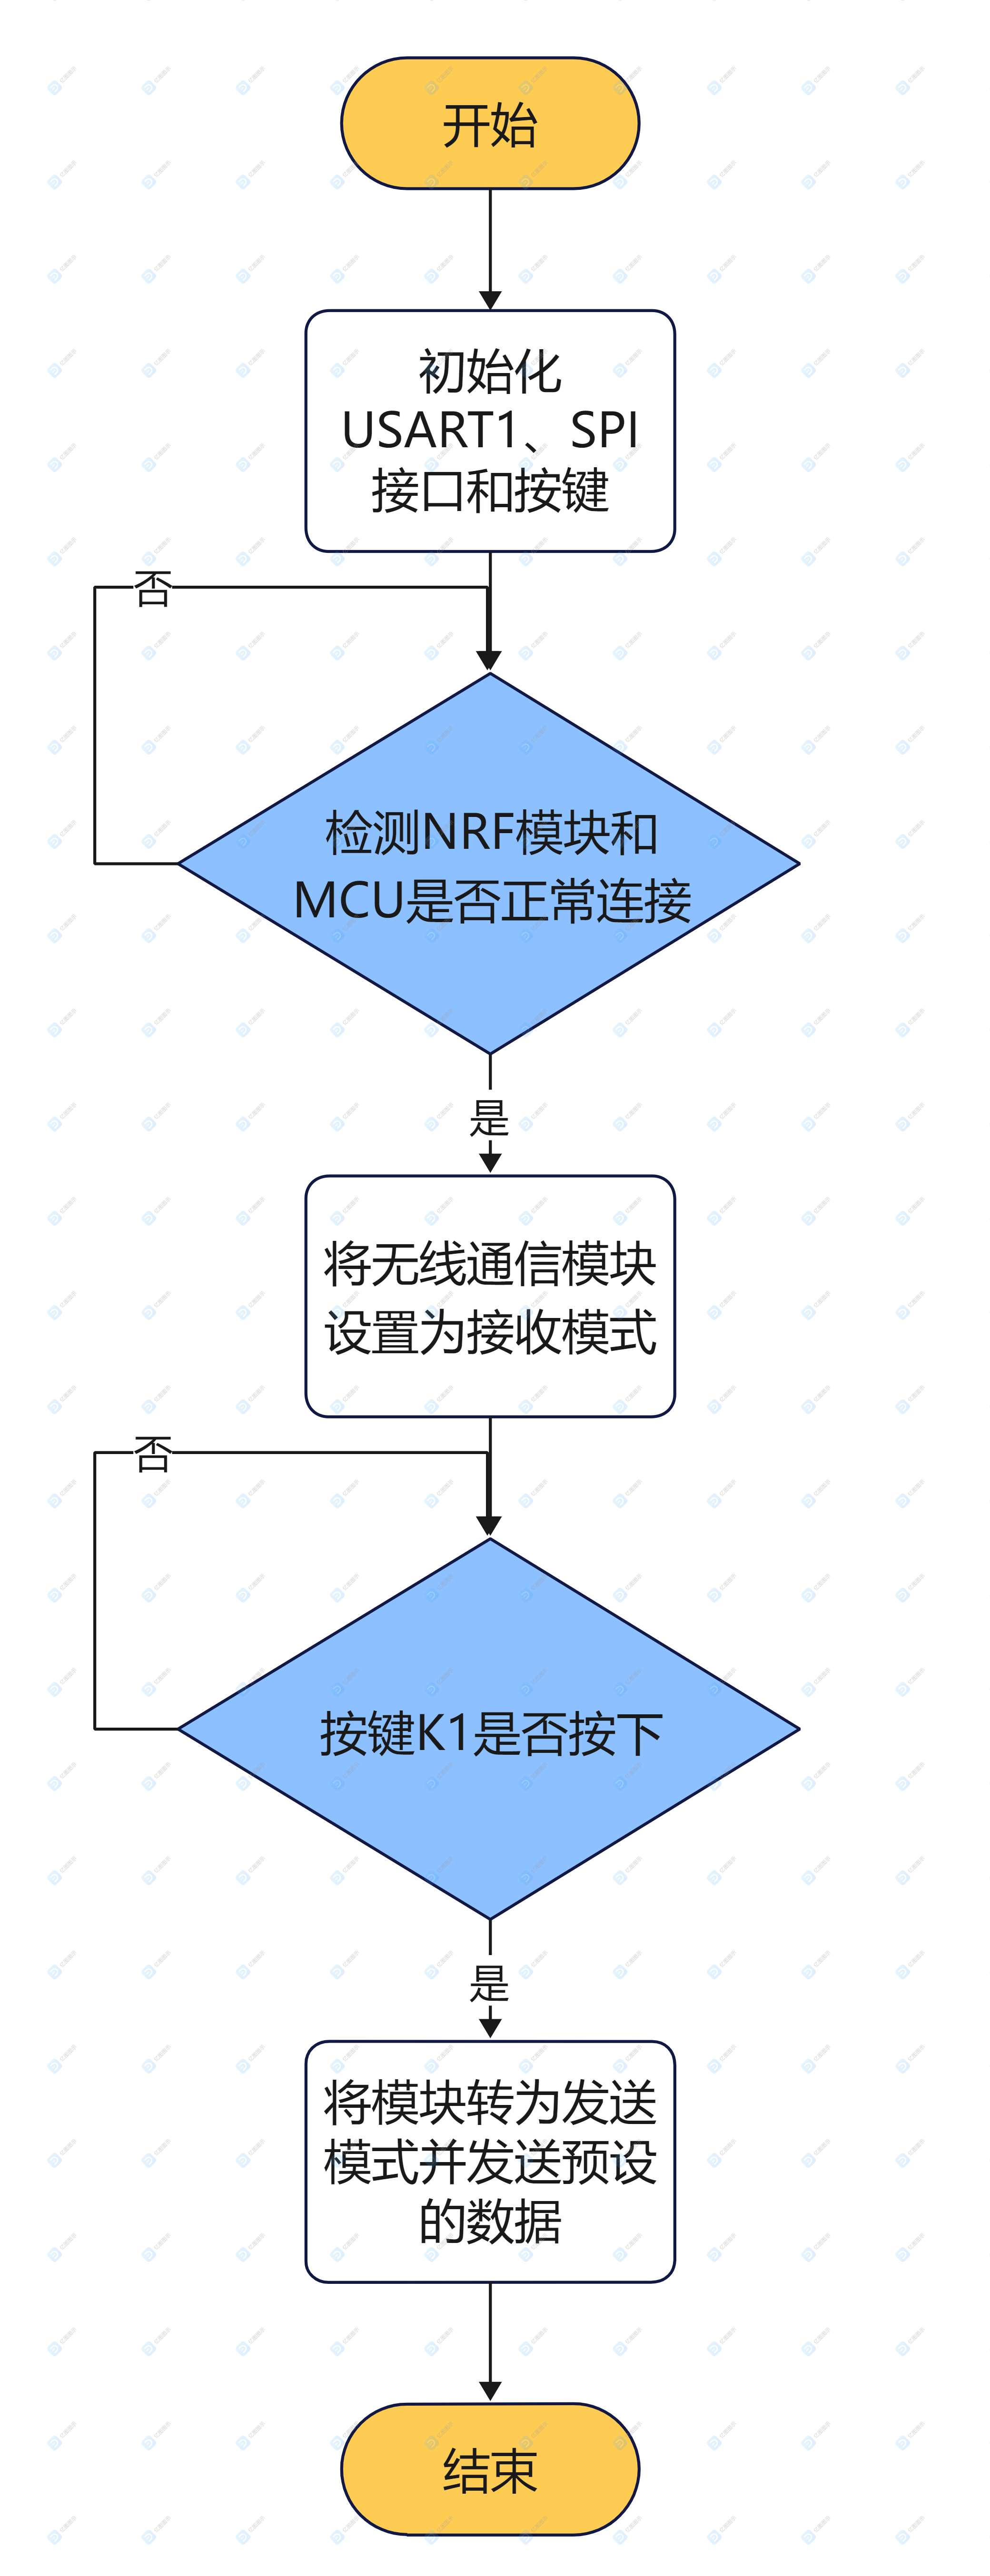
\includegraphics[scale=0.13]{p17.png}
    \caption{主函数流程图}
\end{figure} 

根据我们之前写的各配置文件,我们可以编写出如下的主函数.

\begin{lstlisting}[caption={}]
#include "stm32f10x.h"
#include "bsp_usart1.h"
#include "bsp_spi_nrf.h"
#include "./key/bsp_key.h"  

u8 status = 0;		 //用于判断接收/发送状态
u8 txbuf[32];	 //发送缓冲
u8 rxbuf[32];	 //接收缓冲
u8 i; 

int main(void)
{    
  USART1_Config(); 
  
  SPI_NRF_Init(); 
  
  Key_GPIO_Config();

  printf("\r\n 这是一个 NRF24L01 无线传输实验 \r\n");
  printf("\r\n 这是无线传输 从机端 的反馈信息\r\n");
  printf("\r\n   正在检测NRF与MCU是否正常连接。。。\r\n");

  status = NRF_Check();   		
  if(status == SUCCESS)	   
    printf("\r\n      NRF与MCU连接成功\r\n");  
  else	  
    printf("\r\n   请检测NRF与MCU是否正常连接。。。\r\n");
  
  printf("\r\n NRF进入接收模式,按 K1 发送数据\r\n"); 


  for(i=0;i<32;i++)
  {	
    txbuf[i] = i; 
  }
  
  NRF_RX_Mode();     // NRF 进入接收模式
  
  while(1)
  {  		 	
    /* 等待接收数据 */
    status = NRF_Rx_Dat(rxbuf);

    /* 判断接收状态 */
    if(status == RX_DR)
    {
      for(i=0;i<32;i++)
      {	
        printf("\r\n 接收数据为:%d \r\n",rxbuf[i]); 
      }
      
      printf("\r\n进入接收模式,按 K1 发送数据\r\n"); 
    }
     
    if (Key_Scan(KEY1_GPIO_PORT, KEY1_GPIO_PIN) == KEY_ON)   
	 // 按键按下,开始送数据
    { 
      /* 发送数据 */
      NRF_TX_Mode();
           
      status = NRF_Tx_Dat(txbuf);
      
      /* 发送数据的状态 */
       if(status == TX_DS)
      {
        printf("\r\n发送数据成功\r\n");
      }
      else
      {
        printf("\r\n发送数据失败  %d\r\n", status);
      }
      
      printf("\r\n 进入接收模式,按 K1 发送数据\r\n"); 

      NRF_RX_Mode();
    }
  } 
}
\end{lstlisting}
\clearpage

\section{实物制作与调试}
如图18所示,将两片NRF24L01分别插入两个单片机,再将两个单片机用USB串口接入电脑。

\begin{figure}[htbp]
    \centering
    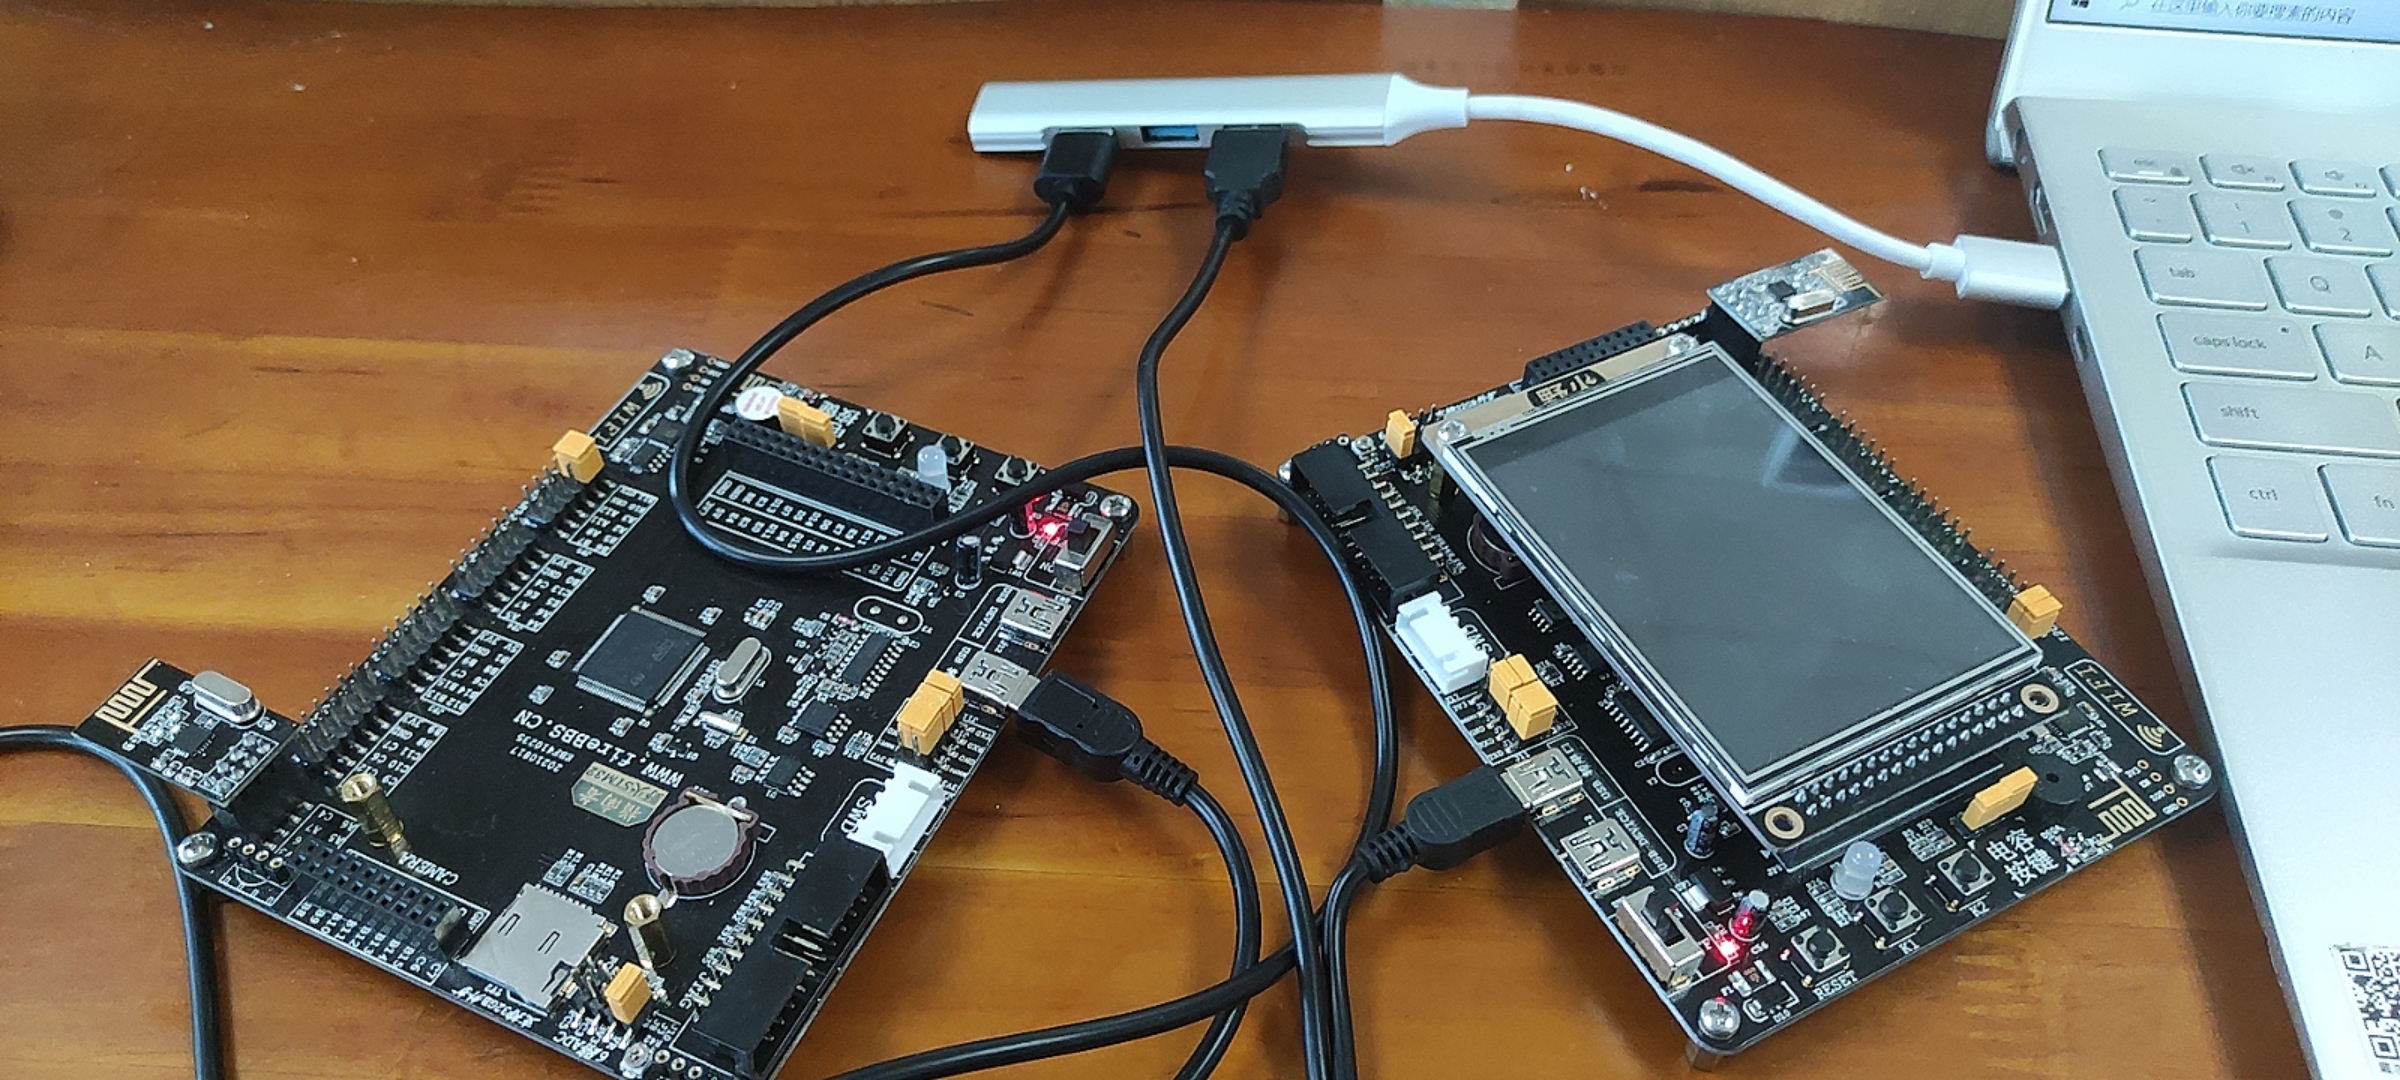
\includegraphics[scale=0.15]{p18.jpg}
    \caption{单片机的接法}
\end{figure} 

打开烧录软件mcuisp,将keil5生成的hex文件分别烧进两个单片机,如图19。

\begin{figure}[htbp]
    \centering
    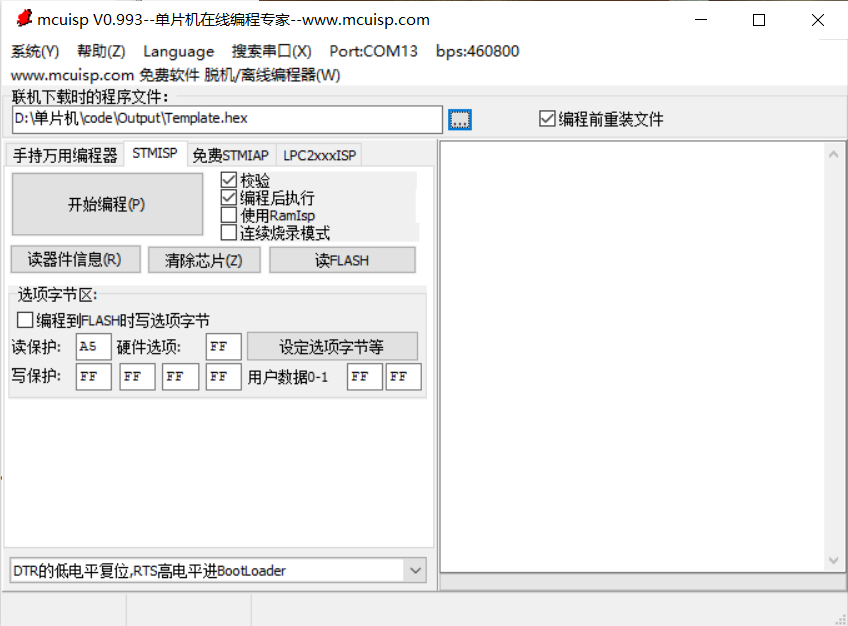
\includegraphics[scale=0.6]{p19.png}
    \caption{通过mcuisp烧入软件}
\end{figure}

先关闭mcuisp(因为如果mcuisp是打开的,串口会被占用,调试助手会无法打开),打开两次串口烧录助手,找准单片机所连接的COM口。打开两个串口,按下第一个单片机的K1。如图20所示,我们预设了一个0-31的数组,可以看到,在COM14的单片机1发送了这个128字节的数据(32个int类型数字),被在COM3的单片机2收到了。

\begin{figure}[htbp]
    \centering
    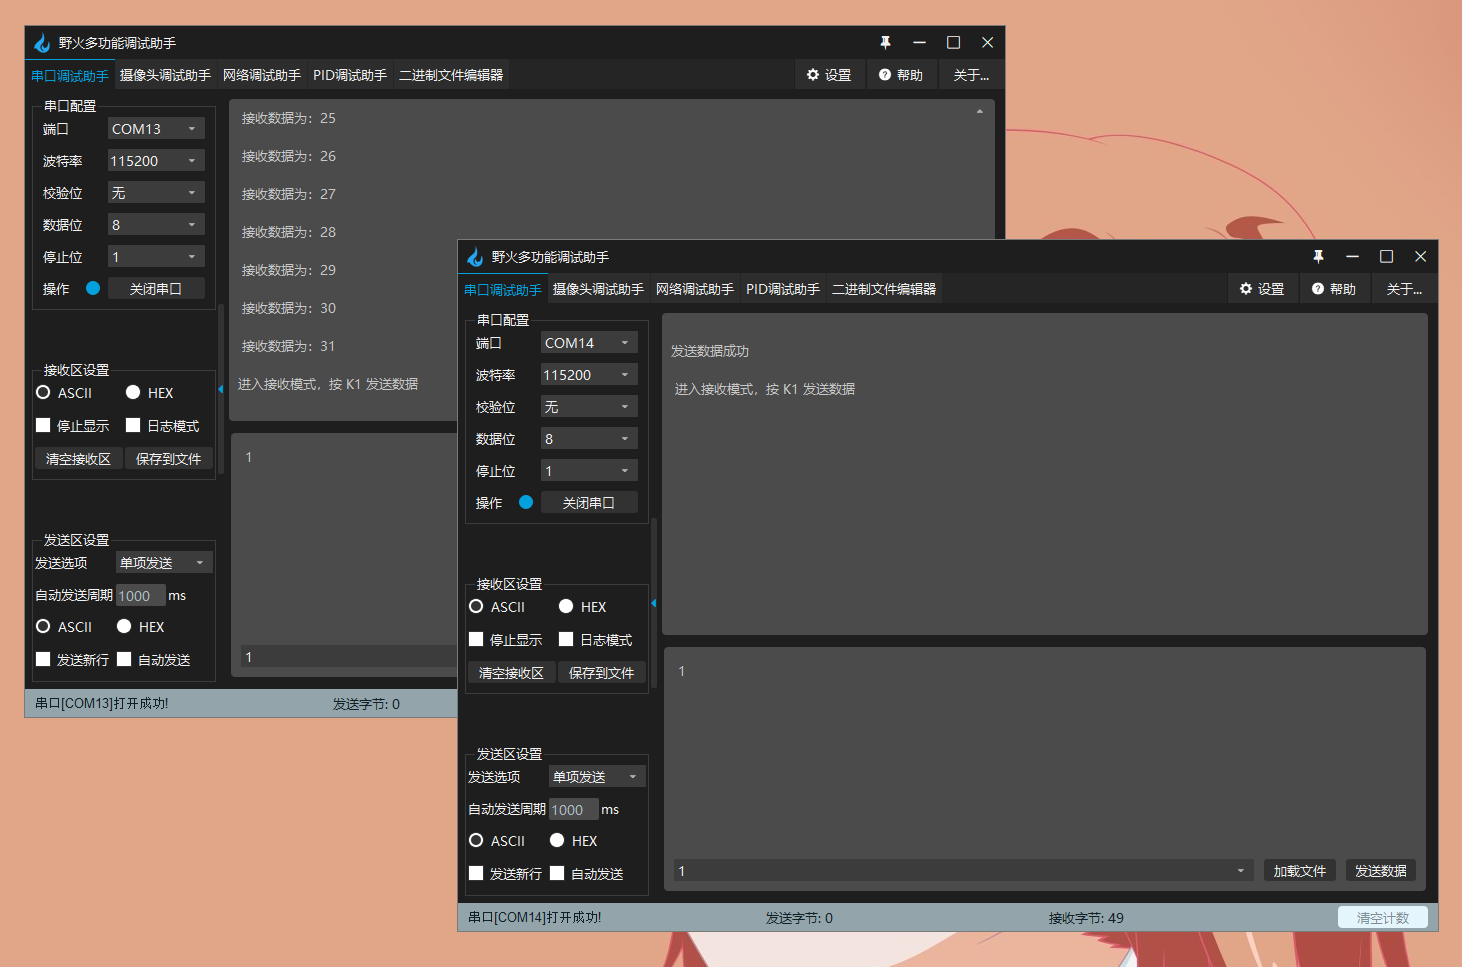
\includegraphics[scale=0.4]{p20.png}
    \caption{单片机1发,单片机2收}
\end{figure}

然后按下单片机2的K1,如图21所示,可以看到,的单片机2发送了这个128字节的数据,被单片机1收到了。

综上所述,两块单片机形成了一组对称的收发系统,达到了预期的目标。
\begin{figure}[htbp]
    \centering
    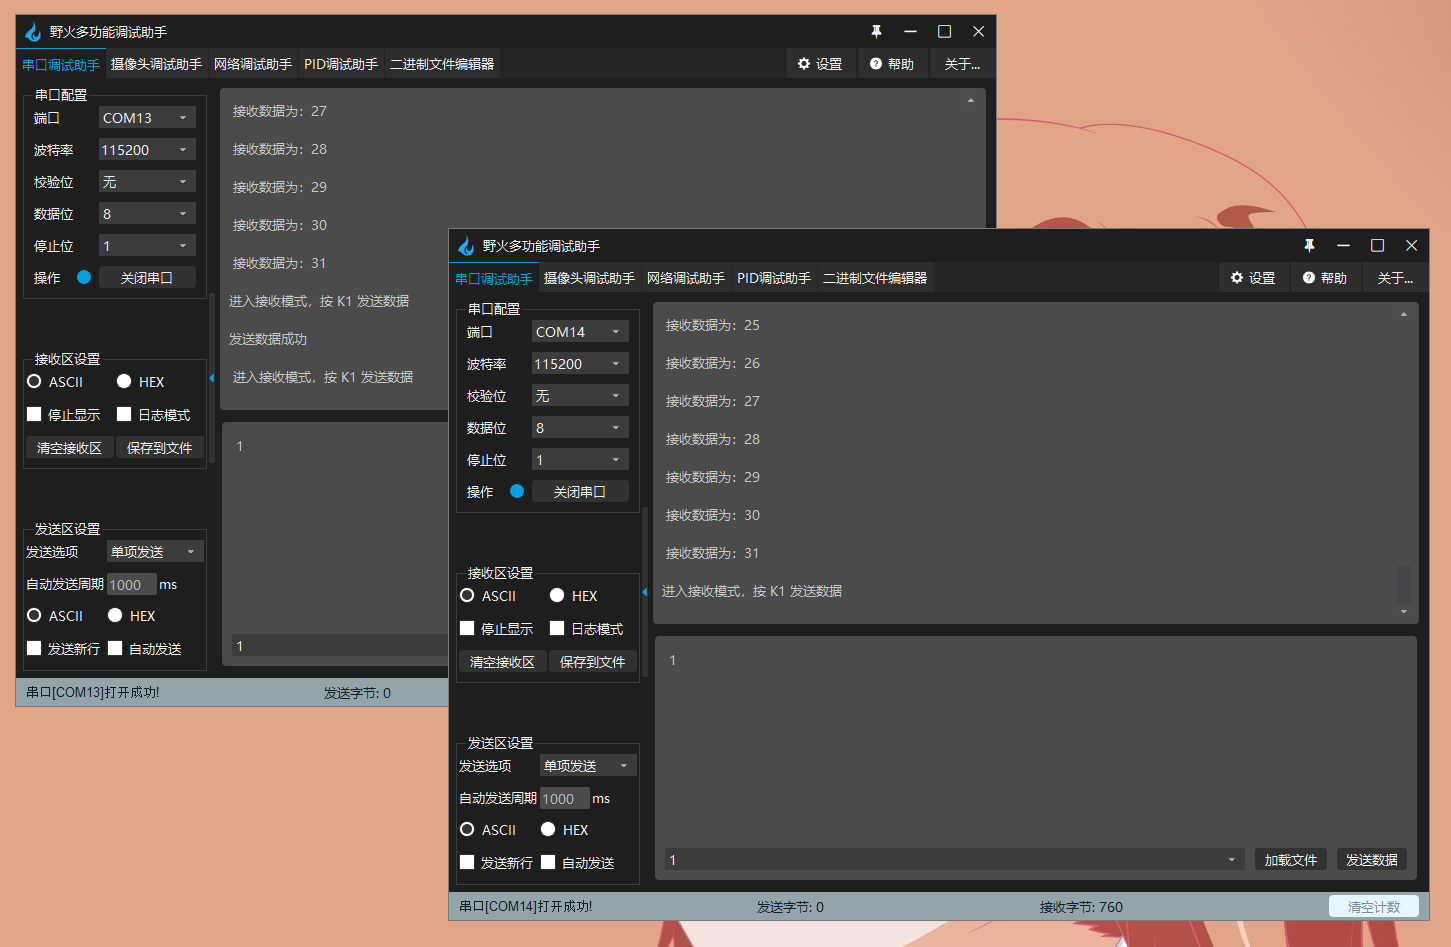
\includegraphics[scale=0.4]{p21.png}
    \caption{单片机2发,单片机1收}
\end{figure}
\clearpage

\section{心得体会}
课程设计的目的之一在于将书本理论知识应用于实际,通过完成这次课设,我不仅巩固了书本所学知识,另外还学到了很多书本中学不到的知识,受益匪浅。

拿到本次设计题目时,由于之前对 NRF24L01 模块没有接触,所以刚开始的时候很茫然,不知从何下手。在查阅大量相关资料后,我意识到芯片手册对于本次课设的完成起着关键性的作用。在认真阅读了芯片手册之后,我逐渐学会了配置这个模块的各个寄存器,调整波特率以及设置工作模式,对无线通信模块 NRF24L01 有了深入的了解。

通过这次课程设计,我的模块化程序设计技能也增强了。通过自创除主函数以外的.c和.h文件,使程序条理更加清晰,可读性更强了。

这次的课程设计是我第一次使用\LaTeX 写的报告,这款排版软件和Microsoft Word相比有很大的不同,它通过类代码的形式进行文档的排版,可以实现”所想即所得“。但也因为\LaTeX 各种库的文件比较复杂,因此学习成本比较高。所以我的这篇报告可能在格式上有一定的问题,希望老师可以谅解。

这次的单片机课程设计使我认识到了做好一份课程设计并不是一件容易的事情。它不仅需要熟悉并掌握教材内容还要有很好的逻辑思维和动手能力,另外还需要查阅相关资料以及自学的能力。虽然过程曲折,但是最终成功实现所有功能,完成了本次课程设计。

\clearpage

\section*{附录}
\addcontentsline{toc}{section}{附录}
这里会展示本设计涉及的库文件。(官方库文件太多,故不做展示,仅展示自己另外写的.h文件)

key.h(按键实现库)
\begin{lstlisting}[caption={}]
#ifndef __KEY_H
#define	__KEY_H

#include "stm32f10x.h"

//  引脚定义
#define    KEY1_GPIO_CLK     RCC_APB2Periph_GPIOA
#define    KEY1_GPIO_PORT    GPIOA			   
#define    KEY1_GPIO_PIN		 GPIO_Pin_0

#define    KEY2_GPIO_CLK     RCC_APB2Periph_GPIOC
#define    KEY2_GPIO_PORT    GPIOC		   
#define    KEY2_GPIO_PIN		  GPIO_Pin_13

#define KEY_ON	1
#define KEY_OFF	0

void Key_GPIO_Config(void);
uint8_t Key_Scan(GPIO_TypeDef* GPIOx,uint16_t GPIO_Pin);

#endif /* __KEY_H */
\end{lstlisting}

usart.h(串口通信库)
\begin{lstlisting}[caption={}]
#ifndef __USART1_H
#define	__USART1_H

#include "stm32f10x.h"
#include <stdio.h>

void USART1_Config(void);
//int fputc(int ch, FILE *f);
//void USART1_printf(USART_TypeDef* USARTx, uint8_t *Data,...);

#endif /* __USART1_H */
\end{lstlisting}

nrf.h(无线通信库)
\begin{lstlisting}[caption={}]
#ifndef __SPI_NRF_H
#define __SPI_NRF_H

#include "stm32f10x.h"

#define TX_ADR_WIDTH 	5  	//发射地址宽度
#define TX_PLOAD_WIDTH  32   
#define RX_ADR_WIDTH    5
#define RX_PLOAD_WIDTH  32 

#define CHANAL 40	//频道选择 

#define NRF_READ_REG    0x00  // Define read command to register
#define NRF_WRITE_REG   0x20  // Define write command to register
#define RD_RX_PLOAD 0x61  // Define RX payload register address
#define WR_TX_PLOAD 0xA0  // Define TX payload register address
#define FLUSH_TX    0xE1  // Define flush TX register command
#define FLUSH_RX    0xE2  // Define flush RX register command
#define REUSE_TX_PL 0xE3  // Define reuse TX payload register command
#define NOP         0xFF  // Define No Operation, might be used to read status register

#define CONFIG      0x00  // 'Config' register address
#define EN_AA       0x01  // 'Enable Auto Acknowledgment' register address
#define EN_RXADDR   0x02  // 'Enabled RX addresses' register address
#define SETUP_AW    0x03  // 'Setup address width' register address
#define SETUP_RETR  0x04  // 'Setup Auto. Retrans' register address
#define RF_CH       0x05  // 'RF channel' register address
#define RF_SETUP    0x06  // 'RF setup' register address
#define STATUS      0x07  // 'Status' register address
#define OBSERVE_TX  0x08  // 'Observe TX' register address
#define CD          0x09  // 'Carrier Detect' register address
#define RX_ADDR_P0  0x0A  // 'RX address pipe0' register address
#define RX_ADDR_P1  0x0B  // 'RX address pipe1' register address
#define RX_ADDR_P2  0x0C  // 'RX address pipe2' register address
#define RX_ADDR_P3  0x0D  // 'RX address pipe3' register address
#define RX_ADDR_P4  0x0E  // 'RX address pipe4' register address
#define RX_ADDR_P5  0x0F  // 'RX address pipe5' register address
#define TX_ADDR     0x10  // 'TX address' register address
#define RX_PW_P0    0x11  // 'RX payload width, pipe0' register address
#define RX_PW_P1    0x12  // 'RX payload width, pipe1' register address
#define RX_PW_P2    0x13  // 'RX payload width, pipe2' register address
#define RX_PW_P3    0x14  // 'RX payload width, pipe3' register address
#define RX_PW_P4    0x15  // 'RX payload width, pipe4' register address
#define RX_PW_P5    0x16  // 'RX payload width, pipe5' register address
#define FIFO_STATUS 0x17  // 'FIFO Status Register' register address

#define MAX_RT      0x10 //达到最大重发次数中断标志位
#define TX_DS		0x20 //发送完成中断标志位	  

#define RX_DR		0x40 //接收到数据中断标志位

#define NRF_CSN_GPIO_PORT    GPIOC
#define NRF_CSN_PIN          GPIO_Pin_6
#define NRF_CSN_GPIO_CLK     RCC_APB2Periph_GPIOC

#define NRF_CE_GPIO_PORT    GPIOC
#define NRF_CE_PIN          GPIO_Pin_5
#define NRF_CE_GPIO_CLK     RCC_APB2Periph_GPIOC

#define NRF_IRQ_GPIO_PORT    GPIOC
#define NRF_IRQ_PIN          GPIO_Pin_4
#define NRF_IRQ_GPIO_CLK     RCC_APB2Periph_GPIOC

#define NRF_CSN_HIGH()      GPIO_SetBits(NRF_CSN_GPIO_PORT, NRF_CSN_PIN)
#define NRF_CSN_LOW()       GPIO_ResetBits(NRF_CSN_GPIO_PORT, NRF_CSN_PIN)		        

#define NRF_CE_HIGH()	      GPIO_SetBits(NRF_CE_GPIO_PORT,NRF_CE_PIN)
#define NRF_CE_LOW()	      GPIO_ResetBits(NRF_CE_GPIO_PORT,NRF_CE_PIN)			      

#define NRF_Read_IRQ()		  GPIO_ReadInputDataBit(NRF_IRQ_GPIO_PORT, NRF_IRQ_PIN)  
//中断引脚

void SPI_NRF_Init(void);
u8 SPI_NRF_RW(u8 dat);
u8 SPI_NRF_ReadReg(u8 reg );
u8 SPI_NRF_WriteReg(u8 reg,u8 dat);

u8 SPI_NRF_ReadBuf(u8 reg,u8 *pBuf,u8 bytes);
u8 SPI_NRF_WriteBuf(u8 reg ,u8 *pBuf,u8 bytes);	

void NRF_TX_Mode(void);
void NRF_RX_Mode(void);
u8 NRF_Rx_Dat(u8 *rxbuf);
u8 NRF_Tx_Dat(u8 *txbuf);
u8 NRF_Check(void); 

#endif /* __SPI_NRF_H */ 

\end{lstlisting}
\clearpage

\section*{参考文献}
\addcontentsline{toc}{section}{参考文献}
[1] 刘海洋. \LaTeX 入门[M]. 北京:电子工业出版社,2013

[2] 刘火良,杨森. STM32库开发指南:基于STM32f103[M]. 北京:机械工业出版社,2013

[3] 刘岚. 单片计算机基础及应用[M]. 武汉:武汉理工大学出版社,2017

[4] 谢自美. 电子线路设计·实验·测试[M]. 武汉:华中科技大学出版社,2005

[5] 康华光. 电子技术基础(数字部分)[M]. 北京:高等教育出版社,2014

[6] 刘志平,赵国良. 基于NRF24L01的近距离无线数据传输[J]. 应用科技,2008(03):55-58.

\end{document}
